\def \currentAuthor {} %so kann jederzeit der Autor geändert werden -> wird in der Fusszeile angezeigt.

\chapter{Einleitung}

Das Projekt entstand, als der biologische Bereich der Universität Innsbruck das Thema Entomophagie behandelte. Entomophagie beschreibt den menschlichen Konsum von Insekten, eine Tätigkeit, die im asiatischen Raum gängig ist. Das Ziel von diesem Projekt ist es aufzuzeigen wie simpel und ressourcenschonend die Zucht von Insekten in einem künstlichen automatisierten Lebensraum ist.

\subsubsection{Vorteile}
Massentierhaltung und riesige Monokulturen zerstören das natürliche Ökosystem der Erde, das Problem wird nicht vereinfacht, indem die gesamte Bevölkerung jährlich steigt. Insekten sind nicht nur eine nahrhafte Möglichkeit diese Nachfrage zu erfüllen, sondern sind auch weniger schadhaft für den Planeten.

Ein weiterer Vorteil besteht auch darin das Insekten bei sich daheim züchten kann und dabei auch vergleichsweise kostengünstig bei der Anschaffung bleibt.




\chapter{Projektmanagement}

\section{Metainformationen}

\subsection{Team}
Unser Team bestand ursprünglich aus 4 Personen. Da ein Schüler sich ungeplant vom Team entfernt hat, daher umfasst das Projektteam 3 Schüler. Projektleiter Leonid Hammer sowie die Gruppenmitglieder Florian Tipotsch und Kevin Glatz.



\subsection{Betreuer}
Die Lehrpersonen Stefan Stolz, MSc und Mag. Nina Margreiter erklärten sich bereit dieses Projekt zu betreuen. Herr Professor Stolz betreute den Technischen Teil der Arbeit und Frau Professor Margreiter den betriebswirtschaftlichen Bereich.


\subsection{Partner}
Der Projektpartner ist die technische Universität Innsbruck. Das Projekt umfasst die Erstellung eines Prototypen für einen automatisierten Insektenbrutkasten.


\subsection{Ansprechpartner}
Die Ansprechpartner zu diesem Projekt waren selbstverständlich unsere Projektbetreuer sowie ao. Univ.-Prof. Thorsten Schwerte.




\section{Vorerhebungen}

\def \currentAuthor{Kevin Glatz}
\subsection{Projektzielplan}

In dem Projektzielplan kann man die einzelnen Schritte sehen, die nötig sind, um auf das Endprodukt zu kommen. Die einzelnen Meilensteine werden hier von der Sicht des Produktes in der richtigen Reihenfolge aufgelistet. In unserem Fall spaltet es sich in drei Bereiche auf, da jeder von uns ein Teil des Projektes übernommen hat und in der Theorie sollte am Ende das ganze Produkt entstehen, sobald man die drei fertigen Teile zusammenfügt. 

\begin{figure}
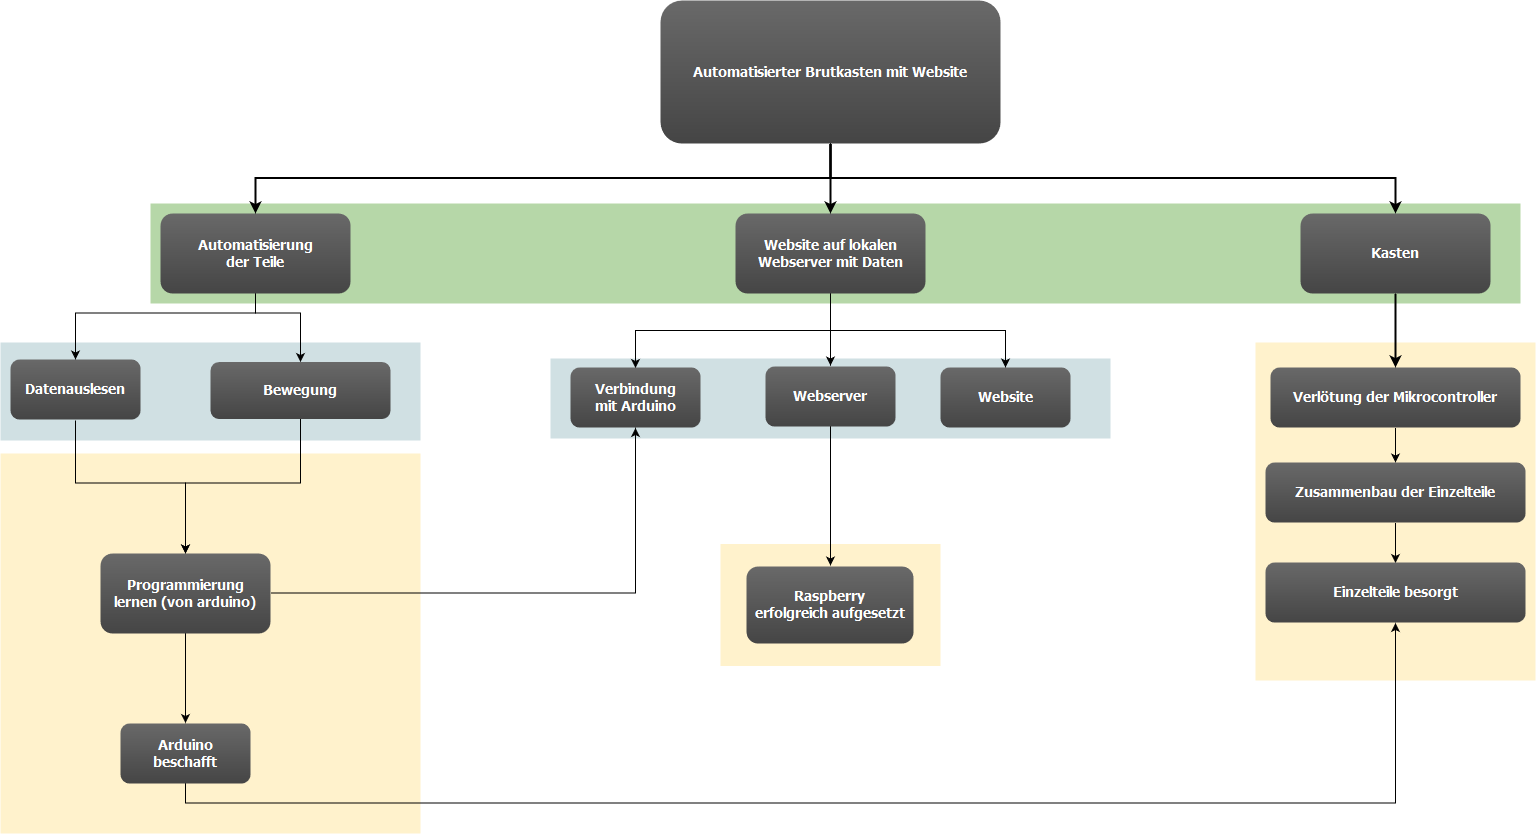
\includegraphics[height=10cm,angle=90]{figures/Zielhierachie}
\caption{Zielplan Hierarchie}
\end{figure}


\newpage
\def \currentAuthor{Kevin Glatz}
\subsection{Risikoanalyse}


\begin{figure}
	\centering
	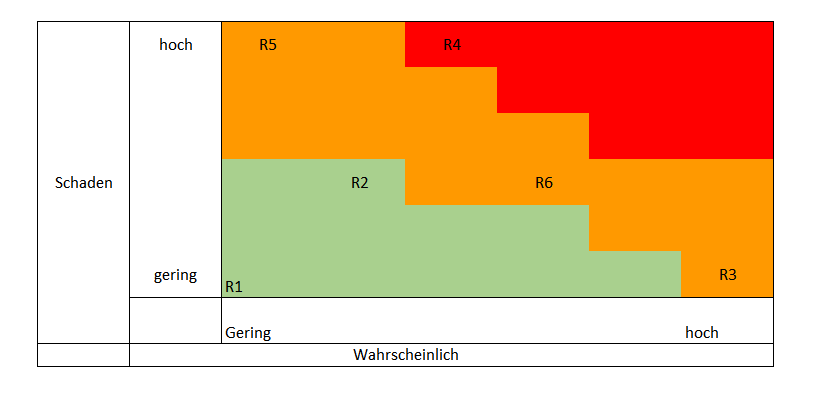
\includegraphics[height=7cm,angle=90]{figures/risiko}
	\caption{Risikomatrix von unserem Projekt}
\end{figure}

Die Risikomatrix ist ein einfaches Tool die Wahrscheinlichkeit und Verheerung von verschiedenen Risiken einfach darzustellen. Je nach Seriosität wird einem Bereich die Farbe rot, gelb oder grün zugewiesen. Schwere und wahrscheinliche Risiken sollten vermieden oder vermindert werden.  Die verschiedenen eingezeichneten Risiken widerspiegeln nicht, was genau das Risiko ist oder wie diese verhindert werden können. In unserer Risikoanalyse haben wir die möglich auftretenden vereinfacht mit R und einer laufenden Nummer betitelt (siehe Abbildung 2.2 Risikomatrix). Diese möchten wir hier nochmals genauer beschreiben:

	R1: Kabel geht kaputt \newline
	Lösung: Kabelpack kaufen damit man Ersatzkabel hat

	R2: Module funktionieren miteinander nicht \newline
	Lösung: Informieren ob alle Einzelteile Synergien 
	
	R3: Projekt wird nicht zeitgerecht fertig\newline
	Lösung:  Meilensteine umformen und evtl. Testzeiten verringern. Länger bzw. intensiver am Projekt arbeiten, um Verspätungen zu verhindern 
	
	R4: Projektpartner ist unzufrieden mit dem Endprodukt. \newline
	Lösung:  Pflichtenheft einholen und eine ständige Kommunikation mit dem Projektpartner aufrecht erhalten. Fortschritte des Projektes vorzeigen um das Projekt auf den Partner anzupassen.
	
	R5: Unterlagen zum Projekt sowie Programmcode oder Diplomarbeit geht verloren \newline
	Lösung: Stets doppelt sichern und auf Github laden das keine wichtigen Daten verloren gehen oder der Datenverlust minimal gehalten wird. 
	 
    R6: Lieferverzug der bestellten Module \newline
	Lösung: Module früh genug liefern lassen damit ein potentieller Verzug keine Folgen hat.  

	



\newpage
\section{Pflichtenheft}
\subsection{Zielbestimmung}
\begin{itemize}
	\item Projektbeschreibung
	\item IST-Zustand
	\item SOLL-Zustand
	\item NICHT-Ziele (Abgrenzungskriterien)
\end{itemize}
\subsection{Produkteinsatz und Umgebung}
\begin{itemize}
	\item Anwendungsgebiet
	\item Zielgruppen
	\item Betriebsbedingungen
	\item Hard-/Softwareumgebung
\end{itemize}
\subsection{Funktionalitäten}
\begin{itemize}
	\item MUSS-Anforderungen
	\begin{itemize}
		\item Funktional
		\item Nicht-funktional
	\end{itemize}
	\item KANN-Anforderungen
	\begin{itemize}
		\item Funktional
		\item Nicht-funktional
	\end{itemize}
\end{itemize}
\subsection{Testszenarien und Testfälle}
\begin{itemize}
	\item Beschreibung der Testmethodik
	\item Testfall 1
	\item Testfall 2
	\item \ldots
\end{itemize}
\subsection{Liefervereinbarung}
\begin{itemize}
	\item Lieferumfang
	\item Modus
	\item Verteilung(Deployment)
\end{itemize}

\newpage
\section{Planung}
\subsection{Projektstrukturplan}
\def \currentAuthor{Florian Tipotsch}
\newpage
\begin{table}[H]
	\centering
	\caption{Projektstrukturplan}
	\label{projektstrukturplan}
	\begin{tabular}{lll}
		P 1   & Projektstart                     &                                \\
		1     & Planung                          & Alle                           \\
		1.1   & Besprechungstermine setzen       & Alle                           \\
		1.1.1 & Vertrag erstellen                & Alle                           \\
		1.2   & Verantwortungsmatrix             & Alle                           \\
		1.3   & Budgetplan erstellen             & Alle                           \\
		2     & Programmierung (Kevin + Flo)     & Kevin Glatz, Florian Tiptsch   \\
		2.1   & Programmiersprache               & Kevin Glatz                    \\
		2.1.1 & Sprache Wählen Š                 & Kevin Glatz                    \\
		2.1.2 & Informationsammlung für Features & Kevin Glatz                    \\
		2.1.3 & Vertraut machen                  & Kevin Glatz                    \\
		2.2   & Arduino UNO kaufen (Flo)         & Florian Tipotsch               \\
		2.2.1 & Vertraut machen                  & Kevin Glatz                    \\
		2.2.2 & Test Programme                   & Kevin Glatz                    \\
		2.3   & Programmierung des Brutkasten    & Kevin Glatz                    \\
		3     & Brutkasten (Leo)                 & Leonid Hammer                  \\
		3.1   & Equipment Liste erstellen        & Leonid Hammer                  \\
		3.1.1 & Equipment überprüfen             & Leonid Hammer                  \\
		3.1.2 & Equipment Kaufen                 & Alle                           \\
		3.2   & Konzeptzeichnung                 & Leonid Hammer                  \\
		3.2.1 & Zeichnen                         & Leonid Hammer                  \\
		3.2.2 & Bauen                            & Leonid Hammer                  \\
		
		4     & Datenbank                        & Kevin Glatz                    \\
		4.1   & ER-Diagramm                      & Florian Tipotsch + Kevin Glatz \\
		4.2   & Sprache Wählen & Florian Tipotsch               \\
		4.3   & HTML Seite mit Daten             & Florian Tipotsch               \\
		5     & Nachforschung (Leo)              & Leonid Hammer                  \\
		5.1   & Welches Tier                     & Leonid Hammer                  \\
		5.2   & Wie viele Tiere                        & Leonid Hammer                  \\
		5.3   & Futter                           & Leonid Hammer                  \\
		6     & Webapp                           & Florian Tipotsch               \\
		6.1   & Prototyp                         & Florian Tipotsch               \\
		6.2   & Login am Server                  & Florian Tipotsch               \\
		6.3   & Registrierung Zuchkammer         & Florian Tipotsch              
	\end{tabular}
\end{table}

\subsection{Meilensteine}

\begin{table}[H]
	\caption{Meilensteine}
	\label{meilensteine}
	\begin{tabular}{lll}
		1   & Planung                      & Alle                         \\
		2   & Programmierung & Kevin Glatz, Florian Tiptsch \\
		3   & Brutkasten             & Leonid Hammer                \\
		4   & Datenbank                    & Kevin Glatz                  \\
		5   & Nachforschung           & Leonid Hammer                \\
		6   & Webapp                       & Florian Tipotsch            
	\end{tabular}
\end{table}

\subsection{Gant-Chart}

\begin{figure}[H]
\hspace*{-2cm}
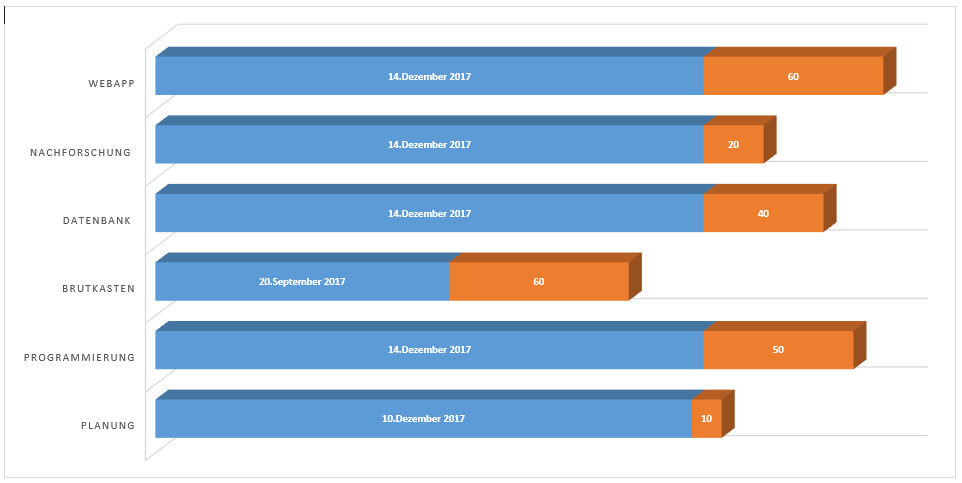
\includegraphics[width=530pt]{figures/Gant}
\caption{Unser Gant Chart für das Projekt} 
\end{figure}
\subsection{Abnahmekriterien}
Die Abnahmekriterien wurden von unserem Auftraggeber so gesetzt, dass es einen Prototypen geben soll, welcher Daten auslesen kann und darauf reagiert.
\subsection{Pläne zur Evaluierung}
Zuerst wollen wird die Daten auf unserem Arduino auslesen und diese dann mit Hilfe eines Wlan Moduls an unsere Website senden.


\chapter{Brutkasten}
\def \currentAuthor{Leonid Hammer}
 Hier werden wir uns dem Aufbau, der Planung und  Ausführung des Brutkastens widmen. 
\section{Equipment Liste}
Um mehr über die einzelnen Komponenten zu erfahren verweisen wir auf eingesetzte Technologien. 
\begin{itemize}
	\item Technisches Equipment
	\begin{itemize}
		\item Arduino Uno
		\item Raspberry 3
		\item Lochrasterleiterplatte
		\item 40-Piece Jumper Wire
		\item Adafruit CCS811 Air Quality Sensor
		\item DHT11 Digital Humidity Temperature Sensor
		\item ESP 8266 WLAN/WiFi Module
		\item Servo Micro 9g SG90
		\item Joystick Dual Axis Module
		\item Raspberry Pi 896 8860 3 Model B
		\item SanDisk Ultra 16 GB SDHC
	\end{itemize}
		\item Baumaterial
	\begin{itemize}
		\item Spanplatten
			\begin{itemize}
			\item Wir benutzen Holz um den Prototyp leichter entwickeln zu können. Da dickeres Plexiglas schwieriger in der Handhabung ist als Holz, da wir doch einige Stellen bearbeiten müssen, die ohne richtiges Werkzeug mühsam wären richtig zu bearbeiten. Spanplatten sind weit verbreitet und werden auf verschiedenste Arten verwendet.
		\end{itemize}
		\item Plexiglas
		\begin{itemize}
			\item Wird hier benutzt um von oben hinein sehen zu können. Diese Scheibe ist mit Scharnieren am Kasten befestigt und kann je nach belieben auch mit einem Schloss gesperrt werden.
		\end{itemize}
		\item Karton
		\begin{itemize}
			\item Karton deshalb um Kleinteile, wie zum Beispiel beim Futterkorb die Luke, anbringen können, da es uns hier die Arbeit um einiges erleichtert. 
		\end{itemize}
	\end{itemize}
\end{itemize}

\section{Überprüfen des Equipments und des Materials}
Ein wichtiger Punkt in Sachen Bestellungen entgegennehmen, ist  die Kontrolle der besagten Materialien. Nachdem die Lieferungen eingetroffen sind, sind auf folgende Punkte zu achten:

\begin{itemize}
	\item Vollständigkeit des bestellten Lieferumfangs
	\item Beschädigungen
	\item wurde das richtige Produkt zugestellt
\end{itemize}

\section{Konzeptzeichnung}
Da unser Brutkasten für eine größere Reichweite von Insekten vertreten sein soll, haben wir auch zwei unterschiedliche Konzeptzeichnungen angefertigt.
\subsection{Zeichnen}


Abbild 4.3 Konzeptzeichnung des Kastens
Zwei Lüftungsklappen die sich automatisiert öffnen je nach Wert des CO² Messgeräts. Boden wird mit Substrat befüllt. 

Die einzigen Nachteile allerdings an diesen beiden Modellen ist, das man die Insekten von Hand ernten muss und nicht einfach am Ende des Tages aus einer großen Box entnehmen kann.

\section{Bauen}

Den Prototypen zu bauen war keine schwere Arbeit. Die Maße sind:
\begin{itemize}
	\item Länge: 50 cm
	\item Breite: 25 cm
	\item Höhe: 30 cm
	\item Dicke des Holz: 0,8 cm 
	\item Dicke des Boden: 1,9 cm
\end{itemize}

Zusammen hält ihn wasserfester Holzleim, damit der Prototyp nicht empfindlich gegenüber Wasserspritzer ist. 

Wir verwenden Spanplatten aufgrund der Kosteneffizienz. Spanplatten werden häufig zurecht geschnitten und man erhält bei größeren Baumärkten Abfall den man sich selber noch einmal zurecht schneiden lassen kann. Zudem lässt es sich mit Spanplatten auch leichter arbeiten als mit einem Holz das eine bestimmte Maserung hat da man hier bei einer zu geringen Dicke ein größeres Risiko des Zerbrechens trägt.

Plexiglas ist ebenso Kostengünstiger als eine herkömmliche Glasscheibe. Ebenso spielt hier die Stabilität wieder eine Rolle. Während Glas höchst zerbrechlich ist, hat hier Plexiglas auch wieder die besseren Voraussetzungen.


\chapter{Eingesetzte Technologien} \label{sec:tech}
\begin{itemize}
	\item Kurzbeschreibung aller Technologien, die verwendet wurden.
	\item Technologien die aus dem Unterricht bekannt sind, nur nennen und deren  Einsatzzweck im Projekt beschreiben, nicht die Technologien selbst.
	\item Technologien die aus dem Unterricht nicht bekannt sind, im Detail beschreiben incl. deren Einsatz im Projekt
	\item Fokus aus eingesetzten Frameworks
\end{itemize}

\newpage	
\def \currentAuthor {Florian Tipotsch}
	\section{Technologie für Webapp}
\begin{itemize}
	\item PHP - Für Webapp
	\item Html - Für Webapp 	
	\item MySql - Für Datenbanken
	\item Yii2 - Für Webapp
	\item MVC - Für Webapp
\end{itemize}
	\subsection{MVC - Model, View, Controller}
	\subsection{Was ist MVC?} \label{sec:mvc}
	MVC, auch Model, View, Controller ist ein modernes Entwurfsmuster das meist für Anwendungen die ein User Interface beinhalten. Zum Beispiel für PHP, JAVA, C\# und Ruby Anwendungen. \cite{MVC}
	\subsection{Vor- und Nachteile}
	\begin{tabular}{ l r }
		Vorteile & Nachteile \\
		Gleichzeitiges Programmieren & Schlechte Übersicht \\
		Hohe Kohäsion \cite{kohaesion} & Konsistente Programmierung notwendig\\
		Lose Kopplung \cite{kopplung} & Steile Lernkurve \\	
	\end{tabular}
	\subsection{Yii2}
	\subsubsection{Was ist Yii}
	Yii ist ein high Performance PHP Framework welches vor allem für die Entwicklung im Web2.0 eingesetzt wird. Web 2.0 fördert die User aktiv im Web mitzumachen. Diese können eigenen Beiträge erstellen und diese auf der Website anzeigen lassen.\cite{Web_2}
	
	\subsubsection{Vor- und Nachteile}
	Yii hat sehr viele Vorteile, allerdings auch einig Nachteile:
	Vorteile sind:
	\begin{itemize}
		\item CRUD-Creator (Gii)
		\item Model Generator (Gii)
		\item Einfache Implementierung von HTML Formulare
		\item Einfach Datenbankzugriffe
	\end{itemize}
	\subsubsection{Gii} \label{sec:gii}
	Gii ist der Yii eigene Model, Crud, Controller, Form, Module und Extension Generator. Mit ihm kann man sehr einfach eine Model Klasse mit einer Unterliegenden Datenbanktabelle erstellen. Aus dieser Model klasse kann man dann wiederum CRUD befehle erzeugen. Mit Gii kann man die gesamte Grund MVC Struktur für Yii2 erzeugen und im weiter verlauf dann nach eigenen Wünschen verändern.
	\subsection{Alternative zu Frameworks}
	Yii kann sehr weitreichend eingesetzt werden. Mit dem richtigen Wissen und Fähigkeiten kann man alles was mit einer PHP Seite möglich ist ganz einfach in Yii2 umsetzten.

Allerdings sind Frameworks nicht Administratoren freundlich da sie sehr viel Vorwissen erfordern um diese richtig zu implementieren. Einfacher zu implementieren sind CMS Systeme. Es gibt sehr viele Große CMS Systeme zum Beispiel:
\begin{itemize}
\item Joomla
\item Wordpress
\item Drupal
\item Contao
\end{itemize}
Diese haben wir auch schon im Unterricht besprochen und damit Websites erstellt. Vorteile sind vor allem die einfache Implementierung und rasche Einrichtung einer Website. Auch SEO wird von den CMS Systemen vereinfacht. Nachteile sind allerdings oft eingeschränkte Möglichkeiten und grenzen welches das CMS setzt.

\subsection{Warum haben wir uns für YII2 entschieden}

Der Hauptgrund warum wir uns gegen CMS Systeme entschieden haben sind die eingeschränkten Möglichkeiten die wir damit hätten. Bei YII2 können wir die gesamte Website nach unseren Bedarf zusammenstellen und auch so bearbeiten wie wir es wollen. Es war uns auch wichtig das wir nach modernen Entwurfsmustern arbeiten. Siehe \nameref{sec:mvc}.

Wir hätten uns auch für andere Frameworks entscheiden können allerdings war uns Yii2 schon bekannt und wir haben damit schon einige Websites erstellt.

Alternativen für Yii2 sind:
\begin{itemize}
	\item PureMVC
	\item Laravel
\end{itemize}
\subsection{PureMVC}
PureMVC ist seit dem Release in 2008 unverändert. Das hat den Vorteil das der administrative aufwand sehr gering ist aufgrund nicht vorhandener Updates. Außerdem muss man das Framework nur einmal lernen und kann dieses dann meistern ohne irgendwelche Änderungen zu befürchten.
Es gibt auch Best-Practicse Beispiele in vielen verschiedenen Sprachen. Diese findet man auf der Website \cite{Pure_MVC}
\subsection{Laravel}
Laravel
\newpage
\def \currentAuthor{Kevin Glatz}
\section{Gas-Sensoren}
\subsection{MQ Gas Sensoren}
Es gibt mehrere MQ Gas Sensoren zum Beispiel:
\begin{itemize}
\item {MQ2}
	Methane, Butane, LPG, smoke
\item {MQ3}
	Alcohol, Ethanol, smoke
\item {MQ4}
	Methane, CNG Gas
\item {MQ5}
	Natural gas, LPG
\item {MQ6}
	LPG, butane gas
\item {MQ7}
	Carbon Monoxide
\item {MQ8}
	Hydrogen Gas
\item {MQ9}
	Carbon Monoxide, flammable gasses
\item Mehr gibt es auf der Website: \cite{MQ_Sensoren}
\end{itemize}
In der Schule haben wir den MQ2 zur Verfügung stehend werden wir auch von der Schule den Adafruit CCS811 bereitgestellt bekommen. Wir bedanken uns dafür vielmals.
\newline
{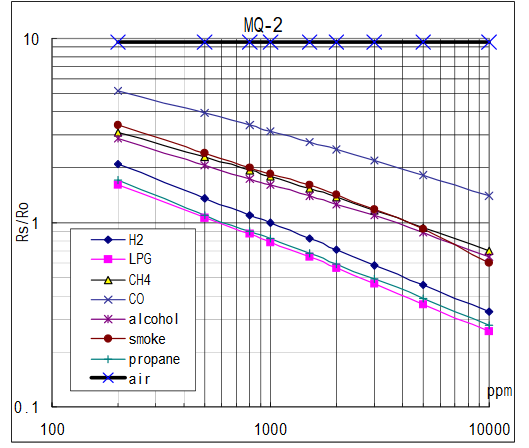
\includegraphics[width=0.8\linewidth]{figures/DatasheetMQ2.png}}{\cite{MQ_Datasheet}}
\cite{MQ_Sensoren}
\newline 
Im Datasheet \cite{MQ_Datasheet} kann man herauslesen das der Sensor MQ2 \cite{MQ_Sensoren} H2, LPG, CH4, CO, Alkohol, Rauch und Propan in einem Bereich von 200 bis 10000 Parts per million (Anteil pro Million) messen kann. Wie empfindlich der Sensor ist, hängt von den RS und RO werten ab.
\begin{itemize}
	\item RS: Sensor Widerstand bei verschiedenen Konzentrationen von Gas
	\item RO: Sensor Widerstand bei 1000ppm von H2 bei sauberer Luft.
\end{itemize}

\subsection{Adafruit CCS811}





\section{Domain-Class-Modelling}
\begin{itemize}
	\item "Dinge" (Rollen, Einheiten, Geräte, Events etc.) identifizieren, um die es im Projekt geht
	\item ER-Modellierung oder Klassendiagramme
	\item Zustandsdiagramme (zur Darstellung des Lebenszyklus von Domain-Klassen darstellen)
\end{itemize}

\section{User-Interface-Design}
\begin{itemize}
	\item Mockups
	\item Wireframes
\end{itemize}

\chapter{Forschung und Findung eines geeigneten Zuchtinsekts}
\def \currentAuthor{Leonid Hammer}
Hier kommt es speziell darauf an, nicht nur ein geeignetes Zuchtinsekt für die Art Prototypen zu finden, sondern nämlich auch heraus zu finden, welche Art von Insekt am Ansprechendsten sein könnte für die Bevölkerung der westlichen Welt.

\section{Verzehr von Insekten}
Entomophagie oder auch, der Verzehr von Insekten, wird bereits in vielen verschiedenen Kulturen betrieben. Nicht nur sind Insekten eine effizientere Nahrungsquelle im Bereich Nahrungsaufnahme, sondern ebenso in der Haltung und Züchtung. Laut Ernährungs- und Landwirtschaftsorganisation der Vereinten Nationen sind die Zahlen der insektenessenden Menschen bereits über 2 Milliarden.

Entomophagie wird hauptsächlich in Afrika, Asien, Mittel und Südamerika sowie bei den australischen Ureinwohnern 

\subsection{Entomophagie in verschiedenen Ländern}
Wie bereits erwähnt wird Entomophagie in einigen Ländern betrieben.
\begin{itemize}
	\item In Australien und Papua-Neuguinea, werden Insekten regelmäßig verspeist. Während es in Australien die Aborigines gibt, die hier verschiedene Larven und von der Honigtopfameise die süße klebrige Masse verspeisen. In Papua-Neuguinea werden Slagowürmer, eine Käferlarve, als Delikatesse bezeichnet.
	\item Afrika, speziell in Nigeria, wird eine Reihe von Insekten regelmäßig verzehrt. Dazu gehören:
	\begin{itemize}
		\item Termiten roh oder gekocht
		\item geröstete Heuschrecken
		\item Palmkäferlarven
		\item Buschmann-Reis, vom Volk San, besteht aus optisch reisähnlichen Puppen verschiedener Termitenarten.
	\end{itemize}
	\item Asien. Hier werden besonders viele Insekten konsumiert. Nicht nur die Vielfalt ist hier größer, sondern auch die Bevölkerung die wesentlich mehr Insekten isst. Unter den auf dem Markt auffindbaren Insekten befinden sich: 
	\begin{itemize}
		\item Wespenlarven, sind in Japan ebenso eine Delikatesse wie Zikaden. Diese werden hier gekocht oder frittiert.
		\item Skorpione, werden meist getrocknet oder angebraten und mit Salz und Pfeffer gewürzt.
		\item Libellen, werden hauptsächlich in Bali verspeist. Die Insekten werden mit Klebestangen gefangen und danach in verschiedenen Saucen gegart.
		\item Schaben, sind in Thailand in den öffentlichen Garküchen anzutreffen ebenso wie Wasserkäfer.
		\item eine Vielzahl von Larven, auf unterschiedlichste Weisen zubereitet. Ob mit Sauce oder frittiert. 
		\item Seidenspinner, nach dem Kochen der Kokons worauf Seide entsteht, verwendet man die Larven in den Kokons weiter als Nahrungsmittel.
	\end{itemize}
	\item Mexiko und Mittelamerika, hier werden Insekten nicht als eine alltägliche Nahrungsquelle bezogen. Hier können Insekten einen höheren Marktpreis erzielen als hochwertiges Fleisch. Ebenfalls benutzen sie Agavenraupen um sie ihrem Agavenschnaps hinzuzufügen, der sich Mezcal nennt. Neben dem Schnaps gelten gekochte Ameisen als eine sehr teure aber delikate Vorspeise, sie wird von vielen als Mexikanischer Kaviar bezeichnet. Darüber hinaus werden Heuschrecken in den südlichen Regionen Mexikos und in Guatemala mit Schokolade überzogen und von Kindern als beliebte Süßspeise angesehen.
	
	\item Südamerika, hier werden vom Rüsselkäfer Suri die Larven verspeist. Neben den Larven gibt es noch Hormigas Culonas, übersetzt dickarschige Ameisen. Diese werden hier gebraten und verspeist und gelten ebenfalls als Aphrodisiakum. 
	Während Spinnen nicht in den Bereich Entamophagie fallen, da sie keine Insekten sondern Arachnophoben sind, werden in Teilen Südamerikas wo sich hauptsächlich Ureinwohner aufhalten, das Aussaugen einer lebendigen Riesenspinne als Delikatesse gesehen. Sie sind zu vergleichen wie mit dem Verzehr roher Austern in Europa.
	
	\item Während in so vielen Ländern Insekten als Delikatesse betrachtet werden, werden hier in Europa bei dem Gedanken Insekten zu verspeisen oft mit einem Ekelgefühl verbunden. Wobei es in Sardinien und Teilen Frankreichs als Delikat angesehen wird wenn sich in bestimmten Käsesorten die Larve einer kleinen Fliege entwickelt. 
	Ebenfalls war bis Mitte des 20. Jahrhunderts in Deutschland und Frankreich eine Maikäfersuppe bekannt. 
	Es wird immer weiter versucht in Deutschland die Menschen davon zu überzeugen, Insekten als Nahrungsmittel aufzunehmen. Bislang jedoch nur mit magerem Erfolg. Ein Interesse besteht laut einer Umfrage der AStA der Universität München. 9000 Studenten nahmen Teil, 28 Prozent der befragten würden gerne einmal Insekten probieren, falls die Mensa sie anbieten würde. Für 57 Prozent würde es keinen Unterschied machen während 22 Prozent der Befragten die Mensa eher meiden würden.
\end{itemize}

Wie man sehen kann, werden in vielen Regionen der Erde bereits Insekten tagtäglich gegessen, ohne dabei einen Ekelgedanken zu haben. Hier in Europa, ist man nicht damit vertraut Insekten als Nahrungsmittel zu betrachten. Wir haben keine Beziehung zwischen Esskultur und Insekten. 

\section{Warum sollten wir Insekten essen?}
Bei dem Gedanken fühlen sich viele Unwohl oder ein Gefühl der Übelkeit kommt ihnen hoch. Wenn man in Betracht zieht das die Massentierhaltung am Effizientesten ist. Es mag effizienter sein wenn man sich am Jahresende den Umsatz ansieht. Nur wie kann etwas effizient sein wenn die andere Methode nur ein Viertel des Futters braucht als bei der Produktion von Rindfleisch. Oder nur ein Hundertstel an Emission ausstößt. 

Zucht von Heuschrecken und Rindern im Vergleich: \\

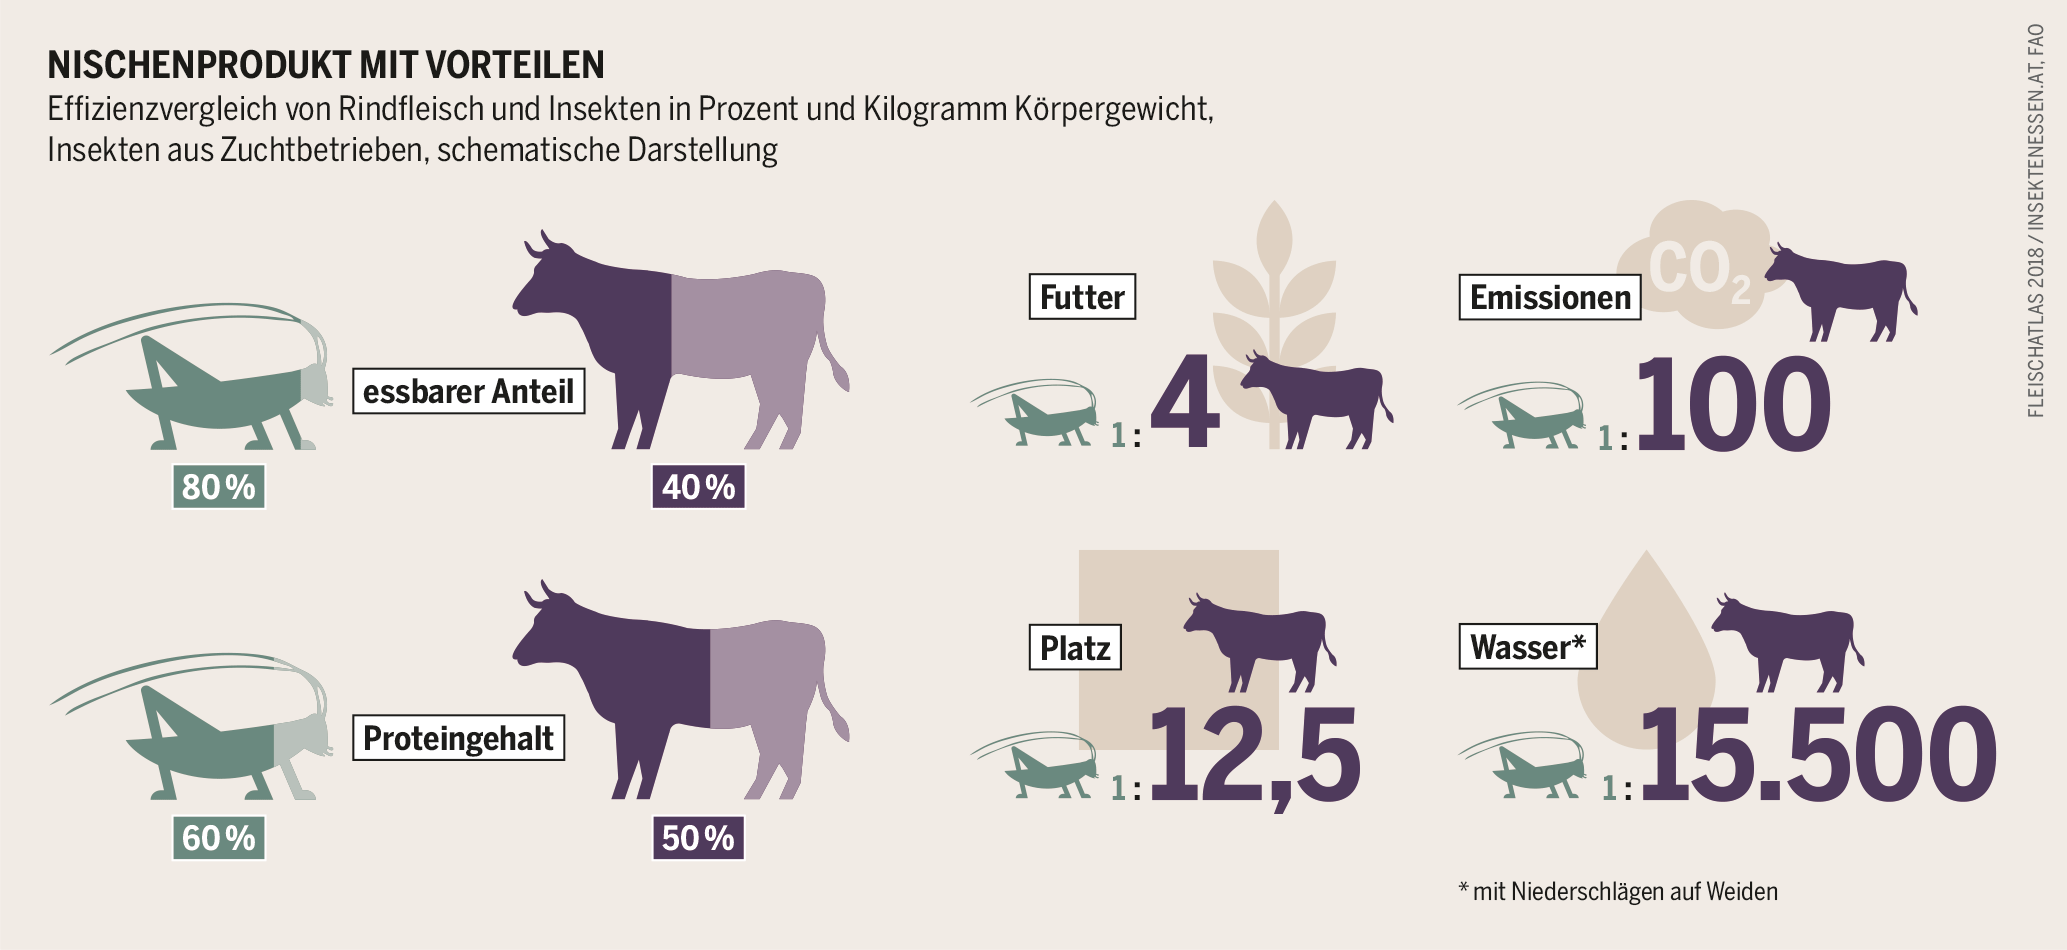
\includegraphics[width=0.9\linewidth]{figures/Vergleich_Mehl_zu_Rind.png}
Abbildung 6.2: Vergleich von Insekten zu Rindfleisch
Quelle: https://www.boell.de/sites/default/files/uploads/2018/01/fleischatlas_2018_grafik_44.png?dimension1=ds_fleischatlas_2018

Wie man sieht ist die Fleischproduktion im Vergleich zur Insektenzucht keineswegs effizienter. Massentierhaltungsstätte sind für 51 Prozent des weltweiten Treibhauseffektes verantwortlich. Sie haben nicht nur einen großen Einfluss auf den Treibhauseffekt sondern ebenfalls auf die Beanspruchung von Futter. Ein Drittel der gesamten angebauten Flächen werden verwendet, um Tiere in Massentierhaltungsstätten zu versorgen. Hinzu kommt noch, das 80 Prozent der weltweit hergestellten Medikamente ebenfalls für diese Stätte genutzt werden. Um zu verhindern dass sich in einer solchen Anlage Krankheiten verbreiten. Unser Fleisch ist also voll von Antibiotika. 
\section{Warum sollten wir Insekten selber züchten?}
Insekten bei sich zu Hause zu züchten ist kein wirklicher Mehraufwand. Je nach Insekt benötigt man anderes Futter, aber im Grunde sind diese alle gleich:
\subsection{Mehlwürmer}
Nicht nur sind sie klein und kaum zu bemerken, sondern sind auch wahre Energiebomben. 
\\ 
auf 100 Gramm:
\begin{itemize}
	\item Energie 550 kcal/ 2303 KJ
	\item Kohlenhydrate: 5,4g - (davon Zucker: 0g)
	\item Ballaststoffe: 6,5g
	\item Protein: 45,1g
	\item Salz: 0,37g
	\item Fette: 37,2g (davon gesättigte Fettsäuren: 9,0g / einfach ungesättigte Fettsäuren: 17,3g /
	mehrfach ungesättigte Fettsäuren: 10,9g)
\end{itemize}

Während Rindfleisch auf 100 Gramm nur:

\begin{itemize}
	\item Energie 139,0 kcal / 582,0 kJ
	\item Kohlenhydrate: 0,0 g
	\item Protein: 22,0 g
	\item Salz: 0,37g
	\item Fette: 4,0 g
\end{itemize}
\\

Hier wir einem schnell bewusst wie viel Energie, Futter und Medikamente verschwendet werden um eine Kuh groß zu ziehen, welche im Endeffekt weniger hergibt als ein kleines unscheinbares Insekt.

\subsubsection{Wie züchtet man Mehlwürmer?}
Besorge Dir zwei Boxen aus Glas oder Kunststoff die glatt ist. Aquarium oder Vorratsbox alles geht. Das Gefäß muss einen Deckel haben. Dieser muss kleine Löcher enthalten. Damit Luft in die Box kommt, die Mehlwürmer aber nicht heraus. Keine Pappe oder Holz verwenden, diese würde von den Tieren zerfressen werden.
\\
Man benötigt ein Substrat das man sich selber aus Getreide und Körnern mischen kann. Dieses Substrat dient als Nahrung der Tiere. Diese gibt es auch zu kaufen im Zoohandel. Das Substrat sollte am Besten noch einmal zermalmt werden, damit es auch die Larven essen können. Das Substrat sollte mindestens 6 cm hoch auf den Boden verteilt werden. 
\\
Es gibt aber auch Knochenmehl als Futter für die Tiere, von diesem ist abzuraten für die Tiere selber und erst recht wenn man plant die Tiere selber zu essen. 
\\ 
Das Futter besteht im Bestenfall aus trockenen Früchten oder Gemüse. Karottenschalen die man übrig hat eignen sich hervorragen für die Tiere. Wobei sich Weizenkleie und Haferflocken ebenfalls perfekt als Futter für die Tiere eignen. 
Trockenes Futter da es sonst in der Wohnung zu unangenehmen Gerüchen kommen kann, da das Obst oder Gemüse schlecht wird. 
Die Tiere sollten jeden zweiten Tag gefüttert werden oder man wechselt das Gemüse beziehungsweise das Obst sobald es anfängt schlecht werden.
\\ 
Es kann bis zu 10 Wochen dauern bis sich die Mehlwürmer vermehren. Außerdem ist es zu Empfehlen einen Kilogramm Mehlwürmer zu kaufen und für die Zucht anfangs zu benutzen. 

\subsection{Heuschrecken}
Heuschrecken sind in der Zucht schwieriger als Mehlwürmer. Es Bedarf oftmals mehr als nur einen Versuch. 
\subsubsection{Wie züchtet man Heuschrecken?}
Hier benötigt man ebenfalls zwei Boxen, idealerweise aus Holz. Es werden zwei Böden benötigt. Wobei beim ersten Boden, der Boden selber aus einem engmaschigen Drahtgeflecht besteht. So kann der Kot der Tiere Sorglos in das Fach unter ihnen fallen.
\\
\\
Für den Boden benötigt man hier ebenfalls ein Substrat. Hier aber aus Torf, Sägemehl und Erde. Wichtig hierbei ist die Keimfreiheit. Man kann das Substrat selber im Backofen bei 100 Grad für 20 Minuten sterilisieren.
\\
\\
Heuschrecken fühlen sich von Wärme stark angezogen, heißt ein Spot mit 40-75 Watt kann hier helfen. Es sollte allerdings keine Kabel in der Zuchtbox selber sein da sonst die Tiere es versuchen würden zu essen. Anfangs reichen 20 erwachsene und geschlechtsreife Heuschrecken wobei davon eine 1 zu 1 Mischung zwischen Männchen und Weibchen sein sollte. 
\\
\\ Für die Eiablage sollte ein kleineres Gefäß zur Verfügung stehen und ebenfalls mit Substrat befüllt sein, es sollte ein wenig feucht sein. 
\\
\\
10 Tage nach der Eiablage sollte man das Gefäß herausnehmen und mit einem Neuen ersetzen. Die frischen Eier in eine andere Zuchtbox hineingeben und am Tag eine Temperatur von 30-35 Grad und auf Nacht eine Temperatur von 20 Grad aussetzen für die bestmögliche Chance des Schlüpfens.

\subsection{Buffalowürmer}
Sie sind in der Triade häufigsten Käferlarven, die als Futtertiere gezüchtet werden, die Kleinsten unter ihnen. Der Buffalowurm bietet gegenüber dem Mehlwurm eine Kürzere Entwicklungszeit und ist daher für manche Personen eher in Betracht zu ziehen.
\subsubsection{Wie züchtet man Buffalowürmer?}
In der Zucht verhalten sie sich ähnlich wie Mehlwürmer. Nur ist es hier wichtiger die Käfer in einem sicher verschließbarem Behälter zu haben, da sie ein Schädling sind.
\\
Die Nahrung ist dieselbe wie bei Mehlwürmern. Ein Substrat am Boden mit einer Höhe von einigen Zentimetern und gegebenenfalls auch Obst und Gemüseabfälle.
\\
Anders allerdings sind sie im Bezug auf ihre Umweltbedingungen. Die optimale Temperatur liegt bei 27-28 Grad. Bei dieser Temperatur schlüpfen die Larven binnen 4-6 Tage aus ihren Eiern. Nach 5 Tagen Puppenruhe schlüpfen die Käfer und sind nach zwei Tagen auch schon wieder Geschlechtsreif.

\section{Wirtschaft: Wie viel kann ein Haushalt durch selber Anbauen einsparen?}
In Österreich werden jährlich rund 105.034 Tonnen Rindfleisch gegessen, Stand 2016. 


\chapter{Systementwurf}

\section{Architektur}
\def \currentAuthor{Florian Tipotsch}
\subsection{Design der Komponenten}

Unsere Webapp ist in Yii2 programmiert und ist deshalb nach dem MVC Muster aufgebaut.
\subsection{MVC - Model, View, Controller}\label{sec:MVC}

\subsubsection{Was ist MVC?} 
MVC, auch Model, View, Controller ist ein modernes Entwurfsmuster, welches meist für Anwendungen, die ein User Interface beinhalten, eingesetzt wird. Zum Beispiel für PHP, JAVA, C\# und Ruby Anwendungen. \cite{MVC}

\subsubsection{Vor- und Nachteile}
\begin{tabular}{ l l }
	Vorteile: & Nachteile: \\
	Gleichzeitiges Programmieren & Schlechte Übersicht \\
	Hohe Kohäsion \cite{kohaesion} & Konsistente Programmierung notwendig\\
	Lose Kopplung \cite{kopplung} & Steile Lernkurve \\	
\end{tabular}

Das MVC Entwurfsmuster ist sehr weit verbreitet und hoch angesehen. Es wird deshalb in den meisten Anwendungen mit User Interface angewandt. Der Grund für die Verwendung dieses Musters sind die vielen Vorteile die es bietet. Außerdem können viele Nachteile über Frameworks behoben werden.

\subsubsection{Aufbau von MVC}
Im Grunde arbeitet MVC mit 3 Klassen:
\begin{itemize}
	\item Modell
	\item View
	\item Controller
\end{itemize}
Die verschiedenen Klassen haben unterschiedliche Aufgaben.

\subsubsection{View}
Die View Klasse ist nur zum Anzeigen der einzelnen Teile des User Interfaces verantwortlich. Bei Webseiten zum Beispiel die Index Seite oder das Login Formular. Außerdem nimmt es alle Benutzer/innen Eingaben entgegen.
\subsubsection{Controller}
Die Controller Klasse steuert die ganze Anwendung. Sie nimmt die User eingaben von der View Klasse entgegen und verarbeitet diese. Außerdem ändert sie auch die View Klasse um andere Seiten anzuzeigen. Sie nimmt auch die Daten von der Modell Klasse entgegen, verarbeitet diese und gibt sie an die View Klasse weiter.
\subsubsection{Modell}
Die Modell Klasse enthält die darzustellenden Daten. Sie ist unabhängig von der View und der Controller Klasse

\subsection{CRUD - Create, Read, Update, Delete} \label{sec:CRUD}

\subsubsection{Was ist CRUD?}
CRUD sind die 4 grundlegenden Aufgaben einer Datenbankanbindung:
\begin{itemize}
	\item Create - Erstellen neuer Datensätze
	\item Read - Auslesen der Datensätze
	\item Update - Aktualisieren von vorhandenen Datensätze
	\item Delete - Löschen von Datensätzen
\end{itemize}
\cite{CRUD}
\newline
CRUD ist für alle Datenbankzugriffe verantwortlich die getätigt werden.


\subsection{Yii2} \label{sec:YII2}

\subsubsection{Was ist Yii}
YII ist ein high Performance PHP Framework welches vor allem für die Entwicklung im Web2.0 eingesetzt wird. Web 2.0 fördert das User aktiv im Web mitmachen. Diese können eigene Beiträge erstellen und diese auf der Website anzeigen lassen.\cite{Web_2}

\subsubsection{Gii} \label{sec:gii}
Gii ist der Yii eigene Model, Crud, Controller, Form, Module und Extension Generator. Mit Gii kann man sehr einfach eine Model Klasse mit einer unterliegenden Datenbanktabelle erstellen. Aus dieser Model Klasse kann man dann wiederum CRUD Befehle erzeugen. Mit Gii kann man die gesamte Grund MVC Struktur für Yii2 erzeugen und im weiterm Verlauf dann nach eigenen Wünschen verändern.

\subsubsection{Vor- und Nachteile}
Yii hat sehr viele Vorteile, allerdings auch einige Nachteile:
\newline
Vorteile sind:

\begin{itemize}
	\item CRUD-Creator (\nameref{sec:gii})
	\item Model Generator (\nameref{sec:gii})
	\item Einfache Implementierung von HTML Formulare
	\item Einfach Datenbankzugriffe
\end{itemize}

Nachteile ist der Hohe Setup-Aufwand und die benötigte Kenntnisse in PHP und SQL, welche allerdings bei fast allen Frameworks von Nöten sind.


\subsection{Benutzerschnittstellen} 

Die Benutzerschnittstelle unseres Brutkasten besteht hauptsächlich über die Webapp. Dort kann man sich anmelden und die Daten für den eigenen Brutkasten auslesen. Um sicherzugehen, dass man nur die eigenen Daten sieht, muss man sich auf der Website mit der Seriennummer, die man beim Kauf eines Kasten erhält, registrieren. Dadurch kann man dann auf die Daten zugreifen, welche für die jeweilige Seriennummer gespeichert sind.
\newline
Wenn man noch nicht registriert wird kann man auf der Website einen Link zu unserem Webshop sehen, den wir allerdings nicht in diesem Projekt erstellen werden da es den Rahmen dieses Projektes Sprengen würde.
\newpage
\subsection{Datenhaltunskonzept}
Hier ist unser ER-Diagramm
	\begin{figure}[H]         
	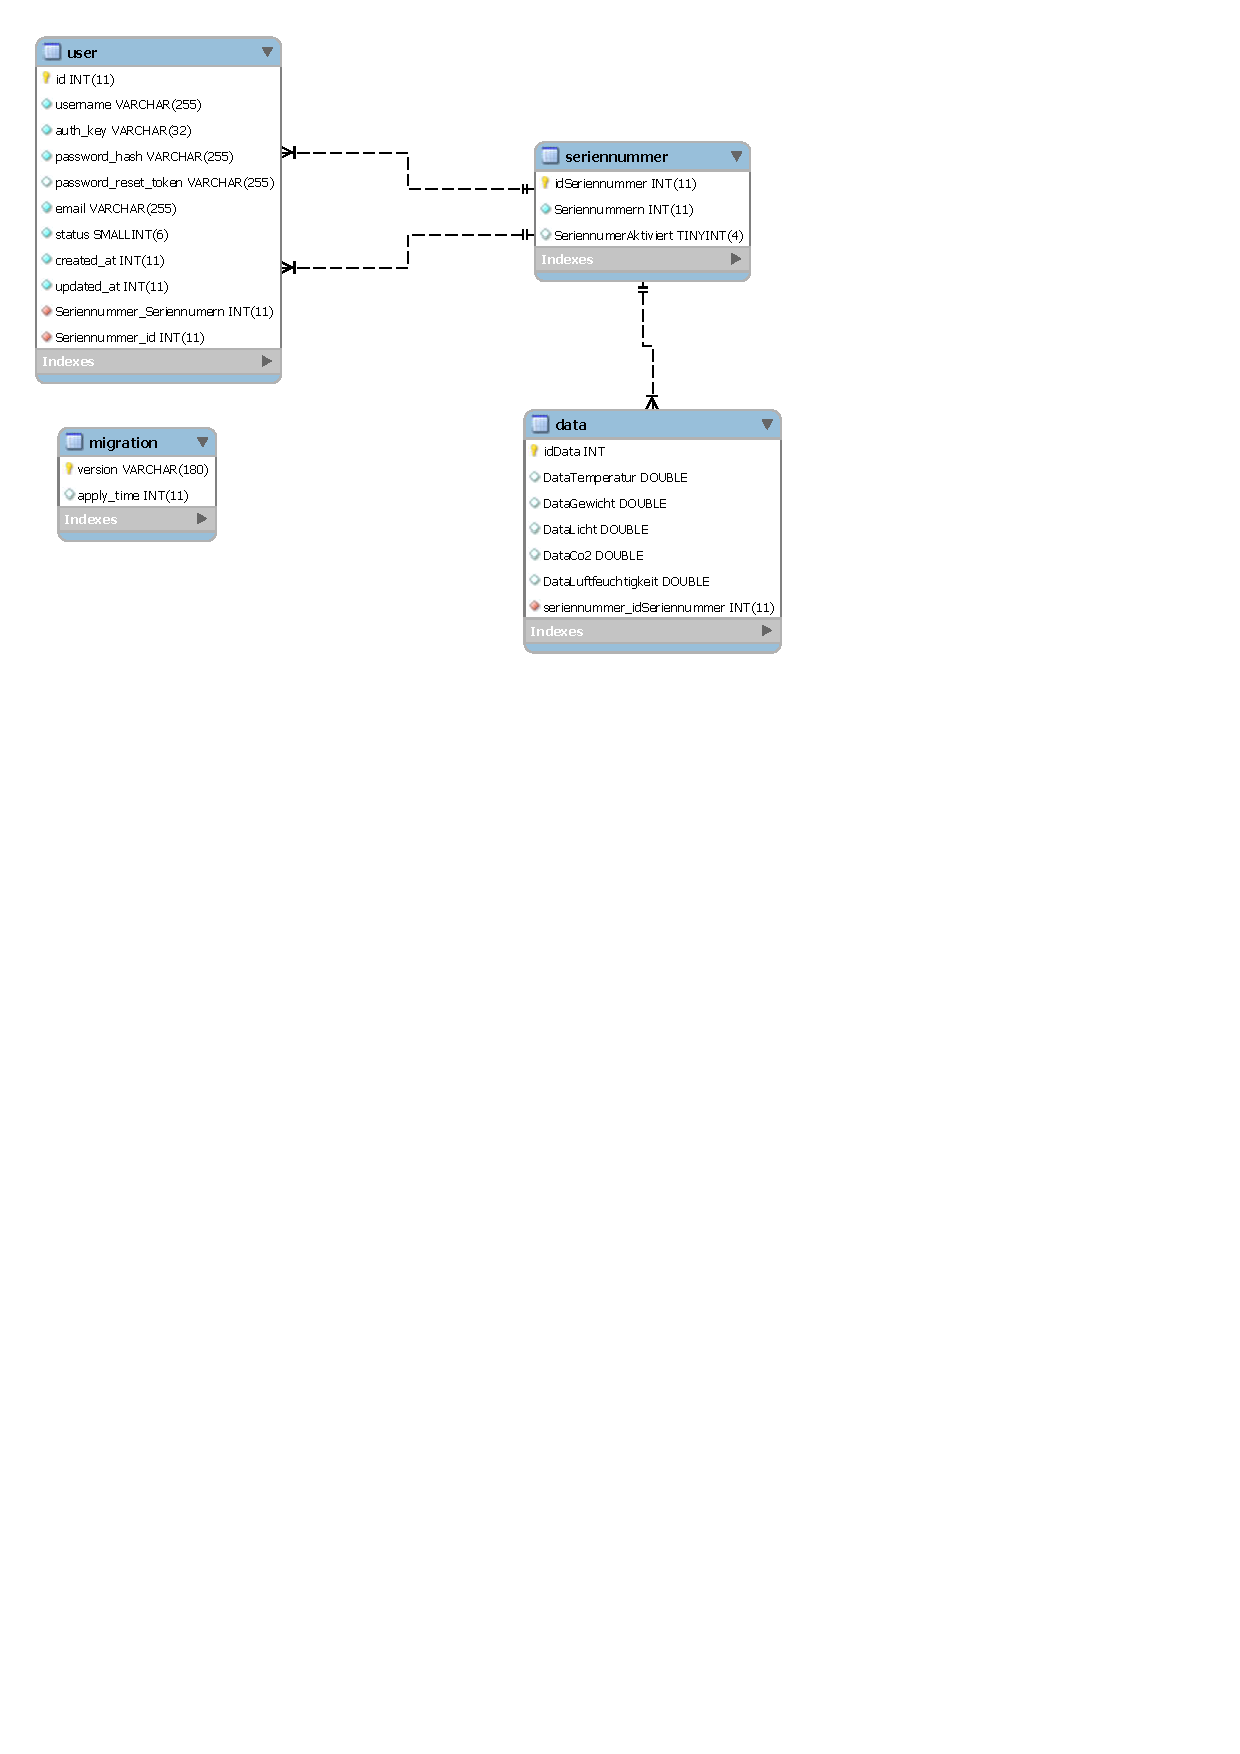
\includegraphics[height=900pt]{figures/ERDiagramm}
	\caption{ERDiagramm unserer Datenbank}
	\end{figure}
	                                                                                                
	Die Datenbank werden wir bei unserem Web Hoster anlegen und dort alle Daten bis zu 7 Tage lang speichern. Daten sollen alle 5-10 Minuten von unserem Brutkasten übermittelt werden. Zur Übermittlung werden wir ein WLAN Modul an unserem Brutkasten anbringen. Mehr dazu im Kapitel \nameref{sec:daten}. Für Prototyp Zwecken werden wir die Daten vorerst lokal über PHPMyAdmin speichern.
	\newpage
	\def \currentAuthor{}

	\newpage
	\def \currentAuthor{Florian Tipotsch}
\subsection{Sicherheitskonzept}                             Auf unsere Website kann man sich mit Hilfe von Username und Password anmelden. Im weiteren Verlauf des Projektes besteht noch die Möglichkeit für unsere Rest-Schnittelle eine Authentifizierung einzubauen. Da unser Prototyp allerdings nur lokal vorhanden ist, ist dies zum jetzigen Zeitpunk noch nicht notwendig.

\subsection{Design der Testumgebung}    
Unser Protoyp wird getestet indem wir ihn einen Tag autonom laufen lassen und am Ende dieser 24 Stunden Periode alle Daten kontrollieren, ob diese Sinn machen und der Realität entsprechen. Um dies zu gewährleisten, bräuchten wir allerdings einen klimaregulierten Raum der CO2 messen kann.

\subsection{Desing der Ausführungsumgebung}                                                                    Das Endprodukt sollte im Freien autonom funktionieren können. Das Setup für den Endbenutzer/in besteht aus dem Anstecken an eine Stromversorgungquelle und dem Verbinden mit dem Internet, sowie das Einsetzen der Insekten. Im weiteren Verlauf der Brutzeit muss der Benutzer/die Benutzerin die Insekten füttern. Unser Produkt übernimmt das Regulieren von Temperatur sowie CO2 Werte, damit die Insekten überleben können.

\section{Detailentwurf}
USE-Cases
Klassendiagramme vom Domain-Klassendiagramm ableiten (incl. detaillierter Darstellung und Verwendung von Vererbungshierarchichen, abstrakten Klassen, Interfaces)
\begin{itemize}
	\item Sequenzdiagramme vom System-Sequenz-Diagramm ableiten
	\item Aktivitätsdiagramme
	\item Detaillierte Zustandsdiagramme für wichtige Klassen
\end{itemize}

Verwendung von CRC-Cards (Class, Responsibilities, Collaboration) für die Klassen
\begin{itemize}
	\item um Verantwortlichkeiten und Zusammenarbeit zwischen Klassen zu definieren und
	\item um auf den Entwurf der Geschäftslogik zu fokussieren
\end{itemize}

Design-Klassen für jeden einzelnen USE-Case können z.B. sein:

\begin{itemize}
	\item UI-Klassen
	\item Data-Access-Klassen
	\item Entity-Klassen (Domain-Klassen)
	\item Controller-Klassen
	\item Business-Logik-Klassen
	\item View-Klassen
\end{itemize}

Optimierung des Entwurfs (Modularisierung, Erweiterbarkeit, Lesbarkeit):

\begin{itemize}
	\item Kopplung optimieren
	\item Kohäsion optimieren
	\item SOLID
	\item Entwurfsmuster einsetzen
\end{itemize}

\newpage
\def \currentAuthor{Kevin Glatz}

\section{Arduino}

Die erfolgreiche Verwendung des Arduino besteht aus zwei  Punkten:
\begin{itemize}
	\item Verkablung der einzelnen Module 
	\item Programmierung
\end{itemize}

Wir können vor allem dem Programmcode um einiges vereinfachen indem wir diesen in drei Unterbereiche aufteilen, wobei jedes Abteil eine fest zugeteilte Aufgabe bekommt. Dasselbe zählt für die Verkablung der einzelnen Module, da diese mit einer strukturierten Farbkodierung übersichtlicher werden.


\subsection{Verkablung}
\begin{figure}[h]
	
	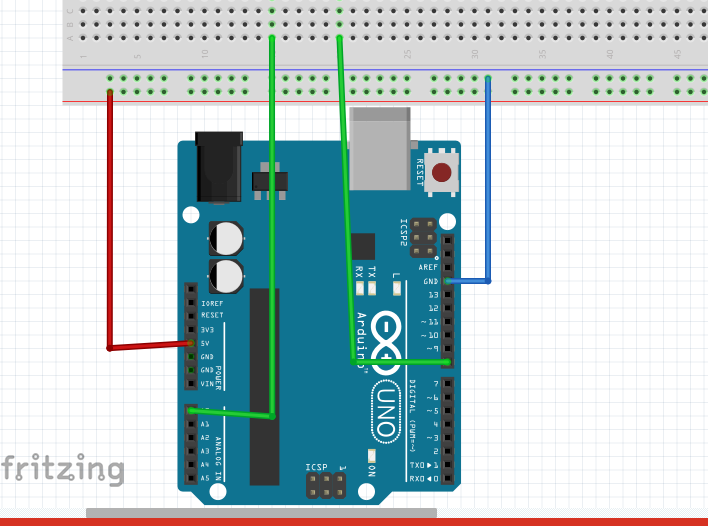
\includegraphics[width=0.7\linewidth]{figures/VerkablungStrukturplan.png}
	\caption{Arduino mit Breadboard}
	\label{fig:verkablungstrukturplan}
\end{figure}

In Abbildung 7.2 können wir nun den Arduino und das Breadboard sehen.  Für eine einfachere Unterscheidung der Kabel verwenden wir ein simples Farbschema. Rot steht für die Stromzufuhr, grün für die Datenauslesung und blau für die Erdung.


Die untersten und obersten zwei Zeilen lassen den Strom bzw. die Erdung horizontal laufen.  Die Steckplätze darüber leiten hingegen jegliche Information vertikal. Ein wichtiges Detail ist das man Stromzufuhr auf der horizontalen Plusreihe platziert (in der Grafik anhand der roten Linie zu sehen), da ansonsten keine Energie ankommt. Bei den vertikalen Steckplätzen gibt es allerdings keine negativ oder positiv gepolten Spalten.

Worauf man bei der Datenauslesung achten muss, ist das Arduino zwei Möglichkeiten dafür verwendet. Zum einen gibt es digitale Daten, welche einen Wert von 1 oder 0 besitzen können. Die Alternative dafür sind analoge Daten, die einen Wert von 0 bis 1023 wahrnehmen können.

Vereinfacht erklärt werden bei digitalen Pins entweder 0 oder 5 Volt gelesen und bei analogen Pins 5 Volt durch 1024 Werte geteilt. Je nachdem wie viel Stromzufuhr das Modul hat, kann es somit einen Datenwert um einiges genauer zurückgeben
\cite{analogRead}




\subsubsection{Bibliotheken importieren und globale Variablen definieren}

In diesem Schritt importieren wir die nötigen Bibliotheken, welche aus GitHub oder direkt von Arduino zur Verfügung gestellt bekommen. Auch werden alle Variablen, die sowohl in den Methoden Setup und Loop verwendet werden erstellt. 

\subsubsection{Setup}

In diesem Schritt importieren wir die nötigen Bibliotheken, welche aus GitHub oder direkt von Arduino zur Verfügung gestellt bekommen. Auch werden alle Variablen, die sowohl in den Methoden Set-up und Loop verwendet werden erstellt.  

\subsubsection{Loop}

Diese Methode verarbeitet und gibt all unsere Werte aus. Besonders an der Klasse Loop ist, dass diese dauerhaft wiederholt wird. Es gibt keine maximale Durchlaufmenge und die Geschwindigkeit eines Durchlaufs wird von der Methode \"delay\" in Millisekunden definiert. Mithilfe dieser Eigenschaften können wir zeitnahe alle Daten auslesen. Falls nun ein Wert eine Mindestgrenze kann, sofort darauf reagiert werden. 

Eine genauere Beschreibung der einzelnen Module und deren Programmierung folgen in den kommenden Seiten


\chapter{Implementierung}
Detaillierte Beschreibung der Implementierung aller Teilkomponenten der Software entlang der zentralsten Use-Cases:

\begin{itemize}
	\item GUI-Implementierung
	\item Controllerlogik
	\item Geschäftslogik
	\item Datenbankzugriffe
\end{itemize}

Detaillierte Beschreibung der Teststrategie (Testdriven Development):

\begin{itemize}
	\item UNIT-Tests (Funktional)
	\item Integrationstests
\end{itemize}

Zu Codesequenzen:
\begin{itemize}
	\item kurze Codesequenzen direkt im Text (mit Zeilnnummern auf die man in der Beschreibung verweisen kann)
	\item lange Codesequenzen in den Anhang (mit Zeilennummer) und darauf verweisen (wie z.B. hier)
	
	
\end{itemize}

\def \currentAuthor {Florian Tipotsch}

\section{Webapp}

Für unser Projekt erstellen wir eine Webapp mit der man die Daten seiner eigenen Zuchtkammer anzeigen lassen kann.
Wir haben geplant, dass man sich mit der Seriennummer des Brutkastens registrieren kann und dann am Handy oder Browser über eine Webapp alle Daten anzeigen lassen kann. Folgende Daten sollte man auslesen können:

\begin{itemize}
	\item Sauerstoff
	\item Luftfeuchtigkeit
	\item Gewicht
	\item Temperatur
	\item Futtermenge
	\item ungefähre Zeit bis zu Reife
\end{itemize}
Als Grundlage für die Website haben wir das Framework Yii2 verwendet. Mehr dazu im Kapitel \nameref{sec:YII2}.

\subsection{Mockups}
\begin{figure}
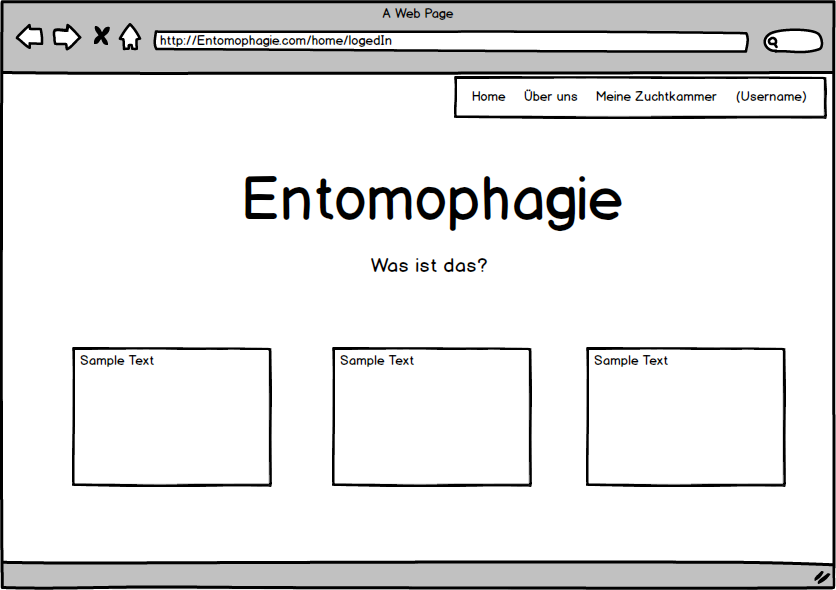
\includegraphics[height=10cm]{figures/Logedin}
\caption{Mockup unserer Seite wenn man eingeloggt ist}
\end{figure}                                                                                                                                                                  Hier sieht man die Ansicht, wenn man auf unserer Website angemeldet ist. Man kann auf die Daten der Zuchtkammer zugreifen indem man auf den Button 'Meine Zuchtkammer' klickt.
\newpage
\begin{figure}
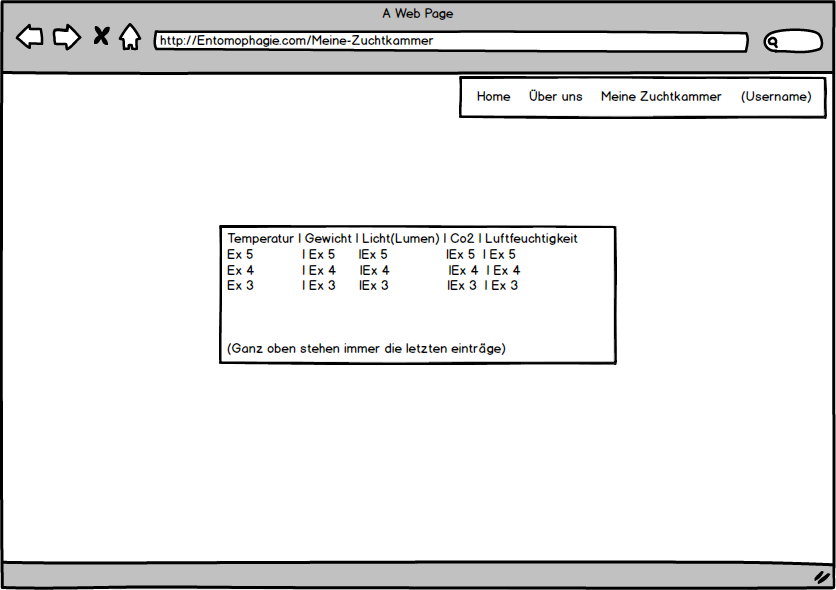
\includegraphics[height=10cm]{figures/Meine-Zuchtkammer}
\caption{Mockup der Seite Meine-Zuchtkammer}
\end{figure}                                                                                                                                                      
Auf der Seite 'Meine Zuchtkammer' sieht man die letzten Daten, die die Zuchtkammer wiedergegeben hat. Diese sind in absteigender Reihenfolge geordnet, was bedeutet, dass der letzte Eintrag ganz oben steht.
\newpage
\begin{figure}
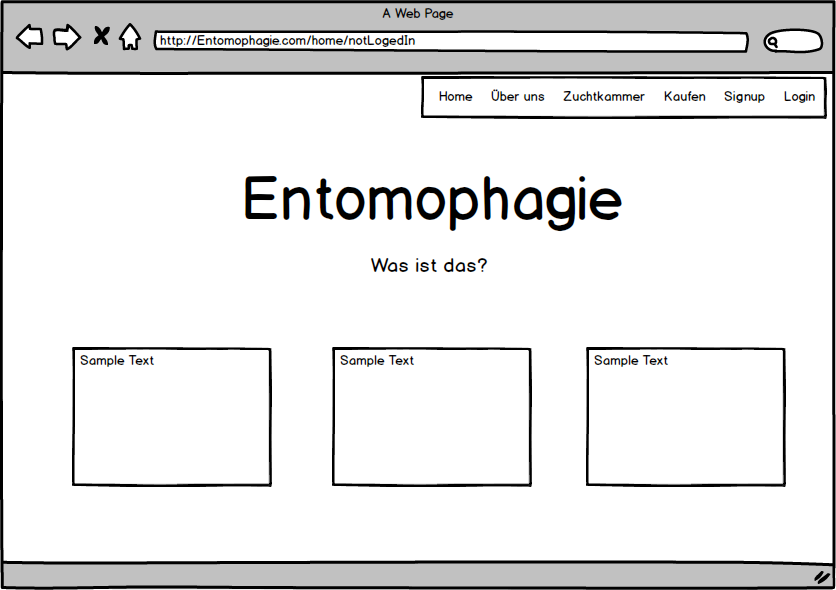
\includegraphics[height=10cm]{figures/NotlogedIN}
\caption{Mockup unserer Seite wenn man nicht eingeloggt ist}
\end{figure}                
Hier sieht man die Ansicht, wenn man auf unserer Website nicht angemeldet ist. Man kann über den Button 'Zuchtkammer' mehr über unsere Zuchtkammern herausfinden. Weiters kann man über den Button 'Kaufen' seine eigene Zuchtkammer erwerben. Über den Button 'Signup' kann man sich als neuer Benutzer registrieren. Um sich registrieren zu können braucht man allerdings zuerst eine Seriennummer, die man beim Kauf einer Zuchtkammer erhält.
\newpage

\subsection{Datenbankzugriffe}                              Unserer Datenbanzugriffe werden von unserem Framework verarbeite. Dabei verwendet das Framework CRUD Befehle und arbeitet nach dem MVC Muster. Das heißt es gibt ein unterliegendes Modell welches Daten an unseren Controller mitgibt, welcher vom View angezeigt werden.

Der gesamte Datenbankzugriff kann mittels Yii2 sehr einfach erstellt werden. Mehr dazu siehe \nameref{sec:gii}.

\subsection{Datenübermittlung} \label{sec:daten}
                                 
Um die Daten von unserem Arduino an unsere Datenbank zu senden werden wir in den Brutkasten ein WLAN Modul einbauen und die Daten alle 5-10 Minuten als JSON-Format an unsere REST-Schnittstelle unserer Webapp senden. Hierfür haben wir das WLAN Modul ESP8266 verwendet. Das hat den Vorteil, dass unsere Daten direkt von unserem Brutkasten an die Datenbank gegeben werden können.
\newline                                                     Für diese Lösung brauchen wir eine REST-Schnittelle in unserer Webapp. Dies kann über Yii2 sehr einfach realisiert werden. Yii2 hat eine vor implementierte REST-Schnittelle, welche man nur noch aktivieren muss. Die Daten werden aus der Modell Klasse ausgelesen und über den Controller an die REST-View weitergeleitet. Die ganze Implementierung sind 5-10 Zeilen Code. Die Code Sequenz sehen Sie im Kapitel \nameref{sec:Rest}.

\subsection{Rest Schnittelle} \label{sec:Rest}
\begin{figure}	
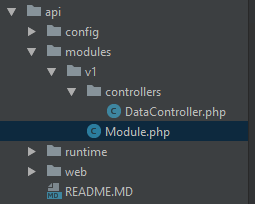
\includegraphics{figures/Ordner}
\caption{Abbildung des API Ordners}
\end{figure}                                                Hier sieht man die Ordnerstruktur. Wir erstellen im obersten Verzeichnis einen neuen Ordner namens 'api' um im Web über folgende \newline URL:'www.entomophagie/api/web/v1/datas' auf unsere REST-Schnittelle zugreifen können. Dabei müssen wir darauf achten, dass wir Groß- und Kleinschreibung beachten. Falls nicht, könnte es passieren, dass wir keine Anzeige bekommen. Um dieses Problem zu lösen, ist es am einfachsten alle Ordner, in unserem Verzeichnis immer klein zu schreiben.\newline
Weiters Kopieren wir 'web', 'config' und den 'runtime' Ordner aus unserem Front- bzw. Backend Ordner. 
\begin{lstlisting}[caption=Controller Klasse für REST]
<?php

namespace api\modules\v1\controllers;
use yii\rest\ActiveController;

class DataController extends Active Controller
{
	public $modelClass = 'common\models\Data';
}
\end{lstlisting}

Hier sieht man die Controller Klasse. In der Controller Klasse müssen wir den Yii eigenen ActiveController einbinden und die Modell Klasse festlegen, welche die Daten ausliest.
\begin{lstlisting}[caption=Module Klasse für REST]
<?php

namespace api\modules\v1;

class Module extends \yii\base\Module
{
public $controllerNamespace = 'api\modules\v1\controllers';

public FUnction init()
{
	parent::init();
}
}
\end{lstlisting}                                                                                                                      
Hier sieht man die Module Klasse. In der Module Klasse wird unser neuer Rest Controller initialisiert, damit unsere Anwendung diesen verwenden kann. Dort müssen wir unseren Controller, den wir zuvor erstellt, haben festlegen.
\newline
Wir haben den Rest Controller mit folgendem Online Tutorial erstellt \cite{Restt}.



\newpage

\def \currentAuthor {Kevin Glatz}
\section{Verkablung}

Die tatsächliche Verkabelung der einzelnen Module war am Anfang recht komplex. Trotz des richtigen Set-ups unterliefen Fehler, die verhinderten, dass Daten sinnvoll ausgelesen werden. Verwendung von Widerständen führte zu falschen oder unrealistischen Daten, da der Strom der darüber lief zu gering bzw. der Widerstand zu hoch war. 

\begin{figure}[h]
	\centering
	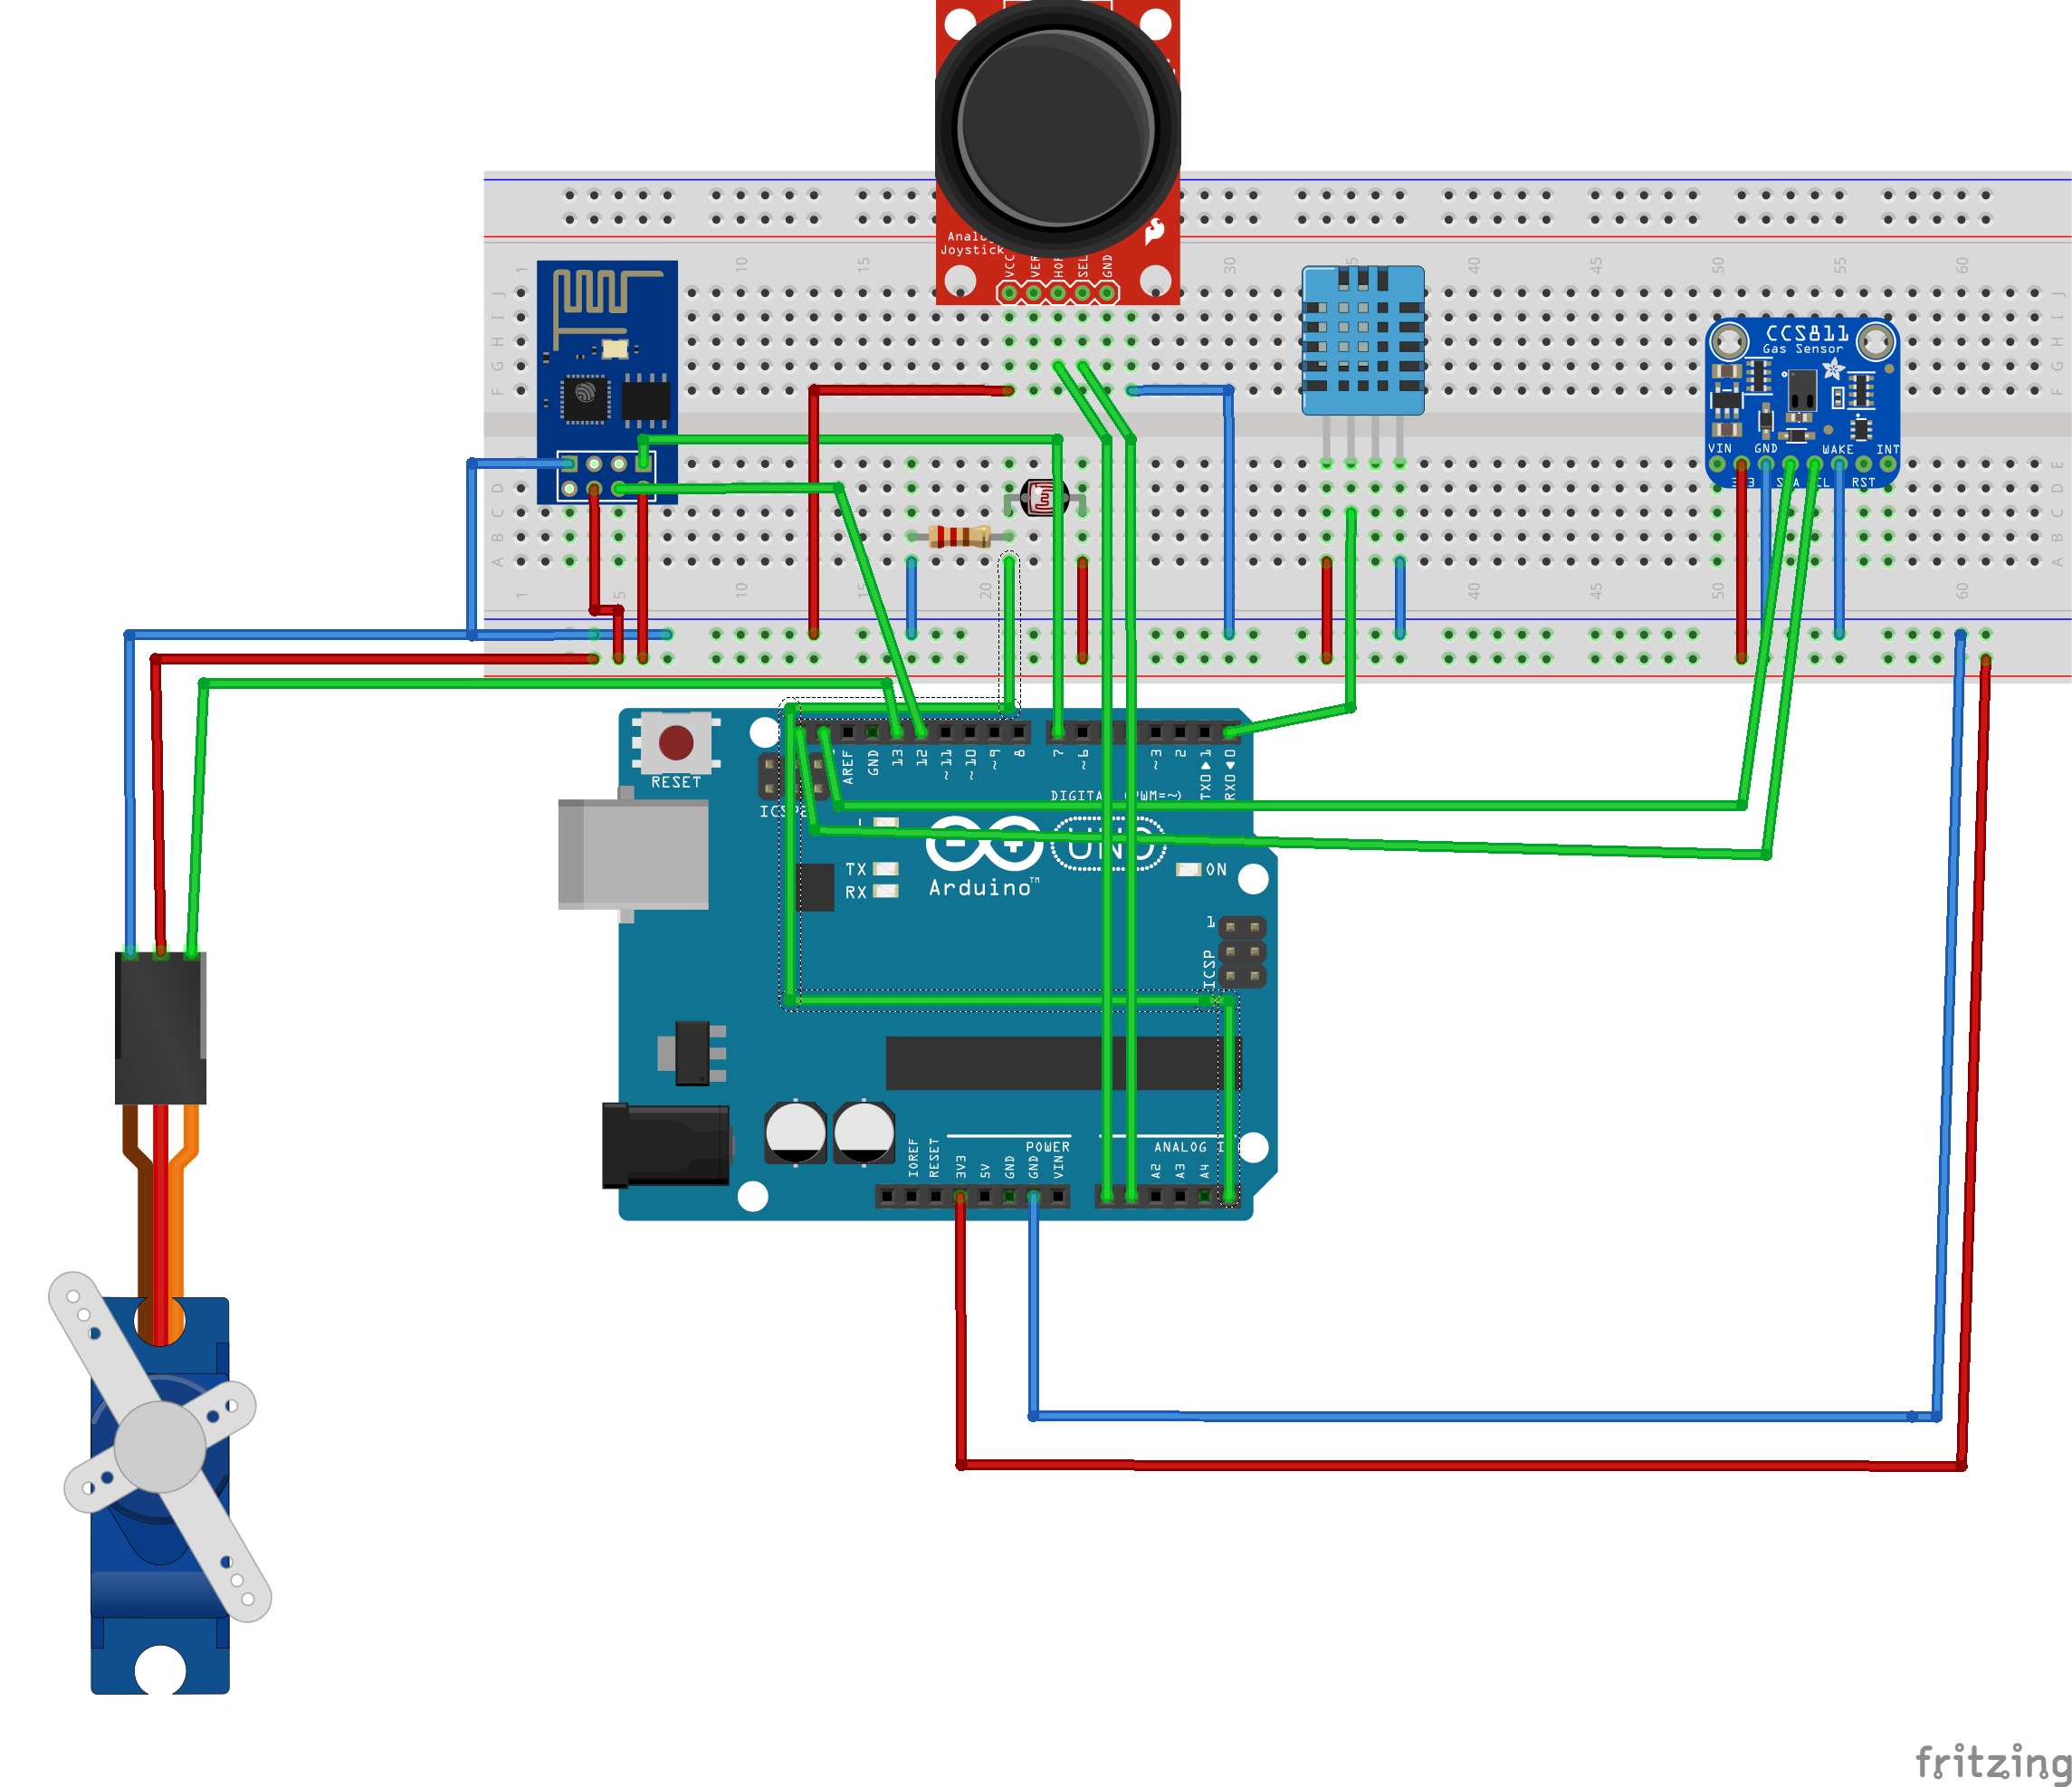
\includegraphics[width=0.7\linewidth]{figures/allMod}
	\caption{Verkablung aller Module}
	\label{fig:allmod}
\end{figure}

In dieser Grafik kann man die Verkabelung aller Module sehen. Abgebildet von links anfangend:

\begin{itemize}
	\item Servomotor SG0
	\item WLAN Modul ESP8266
	\item Joystick Modul (oben)
	\item Lichtempfindlichkeit (unten)
	\item Temperatur und Luftfeuchtigkeitssensor DHT11
	\item CO2 Sensor CCS811
\end{itemize}

Die größte Herausforderung bot der CCS811 sowie der ESP8266, da beide keine typische Verkabelung verwenden. Wie man an der Grafik erkennen kann werden mehrere Strom oder Datenquellen benötigt.

\subsection{CCS811}

\section{Arduino}
Die Verkabelung der einzelnen Module ist aus verschiedenen Gründen wichtig. Zum einen braucht jedes Modul genügend Strom um seine Aufgabe zu erfüllen, gleichzeitig würde es aber ohne die Erdung zu einem Kurzschluss kommen. Des Weiteren ist es wichtig das die Module Daten auslesen und weitersenden können


Der CCS811 benötigt weder digitale noch analoge Werte da er die Pins von der I2C Uhr und Datenlinien verwendet. Es ist auch wichtig anzumerken das dieser Sensor nur mit Mikrocontroller funktioniert die intern I2C "clock streching" unterstützen. In unserem Projekt mussten wir nur die Steckplätze SCL und SDA für den CO2 Sensor verwenden und es funktionierte.

\subsection{ESP8266}

Da der ESP als eingestehende Netzwerkschnittelle zählt, braucht diese besonders viel Energie. Daher muss man beim Verkabeln vor allem darauf achten, dass beide Stromanschlüsse richtig platziert wurden. Ähnlich wie das CO2 Messmodul verwendet der WLAN-Adapter 2 Datenpins. Diese sind allerdings beide digital und können an beliebigen Stellen zwischen 0 und 13 gesetzt werden

\subsection{Joystick Modul}

Der Joystick verwendet ursprünglich zwei analoge Pins und einen Analogen. Damit benötigt dieser Mikrocontroller die meisten Pins. Damit eine Variable X und Y Achse ausgelesen werden kann, benötigen wir die zwei analogen Pins. Der digitale Wert fungiert als Knopfdruck, dieser kann in unserem Projekt allerdings ignoriert werden. Auf die X Ache können wir hingegen nicht verzichten, da beide Werte benötigt werden, um die Position auslesen zu können.



\section{Programmierung}

\subsection{DHT11 \& CCS811}

Für den DHT 11 sowie dem CCS811 gibt es eine von Adafruit frei verwendbare Bibliothek. Mithilfe von dieser kann man ein Objekt erstellen und es mithilfe davon, momentane Temperatur/Luftfeuchtigkeit auslesen.



Der Parameter \#include fügt externe Klassen in unser Projekt ein und erlaubt es uns in das Objekt dht sowie ccs zu erstellen.
Des weitere können wir mit dem Parameter \#define relevante Daten festlegen. Ein solches Beispiel ist, von welchem Pin Daten empfangen werden.


\begin{lstlisting}[language=C, caption=Datenauslesung CCS811, label=code:CCS811read]

delay(2000);
if(ccs.available()){
	if(!ccs.readData()){
		Serial.print("CO2: ");
		Serial.println(ccs.geteCO2());
	}
	else{
		Serial.println("ERROR!");
		//while(1);
	}
}
\end{lstlisting}

\cite{CCS811man}


Die Loop-Funktion, wiederholt sich im vorgegebenen Rhythmus immer wieder und gibt keine Variablen zurück. Dort werden alle Daten ausgelesen und an das WLAN-Modul weitergeschickt bzw. in diesem Fall wird es auf den Serial Monitor ausgegeben.

Die WENN abfrage prüft als Erstes, ob der CO2 Sensor kalibriert wurde oder nicht. Falls es gelungen sein sollte, gibt es die Werte mit dem Befehl Serial.println(ccs.geteCO2()); im Serial Monitor aus.

\subsection{Hebel}

Der Joystick bzw.  der Hebel konnte direkt abgelesen werden. Wichtig hierbei ist es das man nicht nur eine Achse im Setup verwendet, sondern beide, ansonsten kommt es bei dem Loop zu einem Fehler und der Wert von den benötigten Achse verändert sich nicht.


\subsection{SG90}

Die verwendeten Bibliotheken waren bei der Installierung der Arduino eigenen IDE direkt dabei. Der Servo kontrolliert die Luftzufuhr und muss daher Werte vom CCS811 wiederverwenden

\begin{lstlisting}[language=C, caption=Automatisierten Servobewegung bei zu niedrigen CO2 Werten, label=code:SG90]

if(ccs.geteCO2() <= co2Min){
	//move the micro servo from 0 degrees to 180 degrees
	for(;servoAngle < 180; servoAngle++) {       
		servo.write(servoAngle);              
		delay(10);
	} 
} if (ccs.geteCO2() > co2Min && servoAngle != 0){
	servo.write(45); 
	servoAngle = 0;
	Serial.println("RETURN");
}
\end{lstlisting}
\cite{SG90tut}

Die If Abfrage prüft, ob CO2 einen Mindestwert (co2Min) unterschreitet. Falls das passiert wird eine Schleife ausgeführt, die den Servo 180° dreht. Diese 180° würde die Lüftungsklappe aufhalten. Falls der CO2 Wert wieder in einem akzeptablen Bereich liegt und die Position des Motors nicht null beträgt, wird die zweite Schleife aktiviert, die den Motor zur Position 0 zurückbring

\newpage
\def \currentAuthor {Florian Tipotsch}
\newpage
\subsection{Wlan}                                               Für die Implementierung der Wlan-Anbindung haben wir ein ESP8266 verwendet. Das Modul ist sehr einfach einzurichten. Das Ganze haben wir mit den Beispielen von den ESP8266 in der Arduino IDE gemacht.

\subsubsection{ESP8266}                                                                                             
Das Wlan Modul ESP866 wird verwendet um die Verbindung mit dem Internet aufzubauen und die Daten mit Hilfe der REST-Schnittelle an unsere Website senden. Dafür haben wir die ESP8266 Library von Arduino verwendet.\cite{esp8266}
\begin{lstlisting}[caption=Verbindungsaufbau des ESP8266]
	#include <ESP8266.h>
	
	const char* ssid = "SSID des Benutzers";
	const char* password = "password des Benutzers";
	
	const char* host = "Unsere Website";
	
	void setup(){
	Serial.begin(115200);
	dela(10);
	
	Serial.println();
	Serial.println();
	Serial.println("Connecting to ");
	Serial.println(ssid);
	
	
	WiFi.mode(WIFI_STA);
	WiFi.begin(ssid,password);
	}
\end{lstlisting}
                                                                                                       
Hier sieht man den Verbindungsaufbau des ESP8266. In der Zeile 20 wird dann die Verbindung gestartet. Vorher übergeben wir die SSID und das Password des WLANs, womit das Modul sich verbinden soll.
\newpage
\begin{lstlisting}[caption=Verbindungsaufbau Response]
	while(WiFi.status() != WL_CONNECTED) {
	delay(500);
	Serial.print(".");
	}
	
	Serial.println("");
	Serial.println("WiFi connected");
	Serial.println("IP adress: ");
	Serial.println(WiFi.localIP());
	
	


\end{lstlisting}

Bei erfolgreicher Verbindung wird die IP Adresse unseres Moduls ausgegeben.

\begin{lstlisting}[caption=Ausführung der REST Befehle]
client.print(String("GET ) + url + " HTTP/1.1\r\n)" +
	"Host: " + host + "\r\n" + 
	"Connection: close\r\n\r\n");
unsigned long timeout = millis();
while(millis() - timeout > 5000) {
	Serial.println(">>> Client Timeout !");
	client.stop();
	return;
}
\end{lstlisting}
Anschließend können wir in unserer Loop REST Befehle wie Get, Post, Put, etc ausführen.






\newpage
\chapter{Betriebswirtschaftlicher Kontext}


\def \currentAuthor {Kevin Glatz}

                                                                        
\subsection{Arduino in der Wirtschaft}
Mikrocontroller gewinnen vor allem beim Endverbraucher immer mehr an Qualität, allerdings wird auch im landwirtschaftlichen Bereich von diesen Technologien Gebrauch gemacht. In dem Artikel \"Arduino Projekte in der Landwirtschaft und Fischzucht\" wird beschrieben, wie Privatpersonen ihre eigene Lösung zu Problemen wie Fischzucht, Lenksysteme für Erntemaschinen und weitere Fälle gestalten.
Arduino Mikrocontroller werden im wirtschaftlichen Bereich nicht genutzt, da es ein Werkzeug zur Prototyp Erstellung ist. Die einzelnen Module werden hingegen auch im professionellen Raum verwendet.  Der wirtschaftliche Vorteil von Mikrocontroller besteht nicht nur in der Größe, die es für beinahe jeden Bereich verwendbar machen, sondern auch der geringe Preis und die Automatisierung, welche mit dieser Technik ermöglicht wird. Man kann damit nicht nur potenziell Personal sparen, sondern auch permanent Werte einlesen und überwachen. Das erlaubt es uns in der Medizin oder Meerestierforschung schneller einzugreifen falls die Daten einen Mindestwert unterschreiten. Die Kosten dieses Projektes betragen wie folgt, hierzu ist allerdings anzumerken, dass die tatsächlichen Ausgaben um einiges geringer sind. Grund dafür ist, das wir ein Teil der Module schon besetzt haben oder von der Schule zur Verfügung gestellt wurden.



\subsection{Kostenrechnung}

Die Kostenrechnung ist ein mächtiges Werkzeug, welches mehrere wichtige Aufgabenbereiche deckt. Dazu zählen unter anderem Grundlagen der Preisbildung, Verwendung als Entscheidungsinstrument oder auch als Planungsinstrument. Grundlage für die gängigen Kostenrechnungsarten besteht aus der Istkostenrechnung, diese listet alle tatsächlich angefallenen Kosten eines Produktes oder einer Periode auf. \cite{KORE}

	
\newline
		\caption{Kostenrechnung}
		\label{KORE}
\begin{table}[h]
	\begin{tabular}{lll}
		\centering
		Fichten	Leimholzplatte						 & € 8,97 		                  \\
		Plexiglas                   				 & € 5,49€                        \\
		Arduino Uno							    	 & € 25,94                        \\
		Lochrasterleiterplatte		                 & € 2,65                   	  \\
		40-Piece Jumper Wire 						 & € 6,49						  \\
		Adafruit CCS811 Air Quality Sensor     		 & € 22,98                        \\
		DHT11 Digital Humidity Temperature Sensor    & € 4,99                         \\
		ESP8266 WLAN/WiFi Module		             & € 6,29                         \\
		Servo Micro 9g SG90 						 & € 11,70   					  \\
		Joystick Dual Axis Module                    & € 3,99                  		  \\
		Raspberry Pi 896 8860 3 Model B  			 & € 31,95					      \\
		SanDisk Ultra 16 GB SDHC          			 & € 10,99                        \\
		\\
		Summe										 & € 142,44						  \\
	\end{tabular}
\end{table}

Unsere IST-Kosten betragen momentan also 142,44 Euro. Dieser Preis ist in diesem Fall der Selbstkostenpreis, da dies die Kosten sind, die in der Produktion entstanden sind. Um auf einen sinnvollen Verkaufspreis zu kommen führen Unternehmen die sogenannte Absatzkalkulation durch. Diese rechnet Sonderkosten, Gewinne aber auch Rabatte und Skonto mit ein um das fertige Produkt für den maximalen Gewinn zu verkaufen. 



Ein Beispiel eines kommerziellen Brutkasten wäre "The Hive" von livinFarms. Das fertige Produkt produziert ein automatisiertes Ökosystem in dem die Insekten überleben können. Beim Preis unterscheiden sich das Produkt von livinFarms und unsere Arbeit allerdings sehr stark.  "The Hive" ist momentan mit 699 USD beworben. Dieser Preis kann allerdings noch varrieren da dieser kommerzielle Brutkasten selbst noch in der ersten Verkaufsphase ist. 



Mit einer professionellen Lösung wie dieser können wir zwar nicht zwingend Mithalten, allerdings kann unser Produkt immer noch an Popularität gewinnen, da wir die Möglichkeit besitzen mit einem geringeren Preis unschlüssige Kunden anzulocken. Mit der niedrigst-Preis-Strategie versucht man eine Ware oder Dienstleistung zu dem geringsten Preis anzubieten um eine hohe Anzahl von Leuten anzulocken. Ein Beispiel dafür wären Discounter die ihre Produkte massenhaft auf Paletten packen und verkaufen. Ähnlich wie Discounter können wir die Module vielfach einkaufen um Rabatte zu gewinnen.





\newpage
\def \currentAuthor {Florian Tipotsch}
\section{Nutzen einer Website}
Es ist für Unternehmer wichtiger eine Website zu besitzen, weil für viele Personen das Internet der erste Ansprechpartner, um Informationen zu erhalten, ist. Dabei ist es sinnvoll, dass man die gewünschte Website schnell und einfach findet. Dafür ist eine gute search engine optimation (SEO) wichtig, damit die Website in Google auf der Ersten Seite angezeigt wird, da die zweite Ergebnis Seite von Google oft ignoriert wird.

Auch in unserem Projekt haben wir eine Website erstellt. Diese ist allerdings eine reine Funktionswebsite. Auf unserer Website kann man vorerst nur Daten seines Brutkastens auslesen. Natürlich könnte die Website noch mit einem Webshop erweitert werden, da dies allerdings den Rahmen des Projektes sprengen würde, haben wir dies nicht gemacht.

Auf Websiten ist es auch wichtig, dass das Unternehmen widergespiegelt wird. Man sollte ein innovatives Corporate Design, falls eines vorhanden ist, anwenden. Denn in der heutigen modernen Zeit ist es für viele der Erste Eindruck vom Unternehmen.

